%\title{Dokumentation}
\documentclass[12pt,fleqn]{book} % Default font size and left-justified equations
%Packages:
\usepackage{geometry} % Ränder
\usepackage{settings/packages/bookabstract} % Abstract für ein Buch
\usepackage[ngerman]{babel} % Alles deutsch
\usepackage[utf8]{inputenc} % Umlaute
\usepackage[T1]{fontenc} % Auch für Umlaute
\usepackage[german=quotes]{csquotes} %Für Zitate, braucht bibtex
\usepackage{xcolor} % Farbdefinitionen

\usepackage{fancyhdr} % Für Header und Footer
\usepackage[]{listings} %Codeblöcke
\usepackage{accsupp} % Bessere Accessability des PDF (z.B. Code ohne Zeilennummern herauskopieren
\usepackage{xcolor} % Farben
\usepackage{blindtext} % Beispieltext
\usepackage[compact]{titlesec} % Überschriften anpassen
\usepackage[scaled]{helvet} % Helvetica laden
\usepackage{lastpage} % Gesamtseitenanzahl ermitteln
\usepackage{tikz} %Z eichnen
\usepackage{microtype} % Text sperren
\usepackage{calc} % Berechnungen bei Maßangaben
\usepackage[colorinlistoftodos,prependcaption,textsize=scriptsize]{todonotes} % todos vermerken
\usepackage{float} %B esseres Positionieren von Bildern
\usepackage[justification=centering]{caption} % Anpassen von Captions
\usepackage{subcaption} %Anpassen von Subcaptions
\usepackage{wrapfig} % Bilder umfließen
\usepackage{parskip} % Leerzeile = Abasatz
\usepackage{changepage} % Ermitteln, ob gerade/ungerade Seite
\usepackage{tocloft} % Inhaltsverzeichnis anpassen
\usepackage{xhfill} %Zeile mit Linie auffüllen
\usepackage{titling} %Titelseite bearbeiten
\usepackage{etoolbox} % Programmiertechnische Tricks
\usepackage{settings/packages/chaptersinlof} % Fügt Kapitelüberschriften ins Abbildungsverzeichnis ein
\usepackage{settings/packages/chaptersinlot} % Fügt Kapitelüberschriften ins Tabellenverzeichnis ein
\usepackage{settings/packages/chaptersinlol} % Fügt Kapitelüberschriften ins Listingverzeichnis ein
\usepackage{hyperref} % Verlinkungen innerhalb des Dokuments
\usepackage[style=alphabetic,sorting=nyt,sortcites=true,autopunct=true,autolang=hyphen,hyperref=true,abbreviate=false,backref=true,backend=biber]{biblatex} % Literaturverzeichnis
\usepackage{colortbl} % Randfarben von Tabellen
\usepackage{xargs} % Use more than one optional parameter in a new commands
\usepackage[export]{adjustbox} % Bilder umrahmen
\usepackage{xparse}

%Glossar
\usepackage{glossaries} 
\setacronymstyle{footnote-sc}
\DeclareDocumentCommand{\newdualentry}{ O{} O{} m m m m } {
  \newglossaryentry{gls-#3}{name={#5},text={#5\glsadd{#3}},
    description={#6},#1
  }
  \makeglossaries
  \newacronym[#2]{#3}{#4}{\glsadd{gls-#3}\glsseeformat{gls-#3}{}}
}
\makeglossaries
\usepackage[xindy]{imakeidx}
\makeindex
\loadglsentries[main]{glossary}

%To Dos
\newcommandx{\unsure}[2][1=]{\todo[linecolor=red,backgroundcolor=red!25,bordercolor=red,#1]{#2}}
\newcommandx{\change}[2][1=]{\todo[linecolor=blue,backgroundcolor=blue!25,bordercolor=blue,#1]{#2}}
\newcommandx{\info}[2][1=]{\todo[linecolor=OliveGreen,backgroundcolor=OliveGreen!25,bordercolor=OliveGreen,#1]{#2}}
\newcommandx{\improvement}[2][1=]{\todo[linecolor=Plum,backgroundcolor=Plum!25,bordercolor=Plum,#1]{#2}}
\newcommandx{\thiswillnotshow}[2][1=]{\todo[disable,#1]{#2}}

%Colors
\definecolor{middlegray}{rgb}{0.5,0.5,0.5}
\definecolor{orange}{rgb}{0.8,0.3,0.3}
\definecolor{lightgray}{rgb}{0.8,0.8,0.8}
\definecolor{yac}{rgb}{0.6,0.6,0.1}
\definecolor{thmgreen}{RGB}{128,186,36}

% Breite von Randnotizen
\setlength{\marginparwidth}{2.8cm}

%Tabellen
\arrayrulecolor{black}
\setlength{\arrayrulewidth}{1pt}

%includes advanced settings
%Überschriften
\titleformat{\chapter}[hang] 
{\normalfont\LARGE\bfseries\sffamily}{\thechapter}{1em}{} % Kapitelüberschrift Optik
\titleformat{\section}[hang] 
{\normalfont\Large\bfseries\sffamily}{\thesection}{1em}{} % Abschnittsüberschrift Optik
\titlespacing*{\section}{0pt}{0.5cm}{-2pt plus 0pt minus 0pt} %Abschnittsüberschrift Abstände
\titleformat{\subsection}[hang] 
{\normalfont\large\bfseries\sffamily}{\thesubsection}{1em}{} %Unterabschnittsüberschrift Optik
\titlespacing*{\subsection}{0pt}{0.5cm plus 2mm minus 2mm}{-3pt plus 0pt minus 0pt} % ... Abstände
\titleformat{\subsubsection}[hang] 
{\normalfont\large\bfseries\sffamily}{\thesubsubsection}{1em}{} %Unterunterabschnittsüberschrift Optik
\titlespacing*{\subsubsection}{0pt}{0.5cm plus 2mm minus 2mm}{-3pt plus 0pt minus 0pt} % .... Abstände
\titleformat{\paragraph}[hang] 
{\normalfont\normalsize\bfseries\sffamily}{}{1em}{} 
\titlespacing*{\paragraph}{0pt}{0.3cm plus 1mm minus 1mm}{0.1cm plus 0pt minus 0pt}

%Captions
\captionsetup{labelfont=sf, labelsep=newline}

%TOC
\renewcommand\cftchapfont{\normalsize\bfseries\sffamily} % Schriftart der Kapitelüberschriften
\renewcommand{\cftchapleader}{~\xrfill[0pt]{1pt}[thmgreen]} % Linien neben Kapitelnamen
\renewcommand{\cftsecleader}{~\cftdotfill{0}} % Linien neben Abschnittsüberschriften
\renewcommand{\cftsubsecleader}{~\cftdotfill{0}} % Linien neben Unterabschnittsüberschriften
\renewcommand{\cfttoctitlefont}{\sffamily\bfseries\LARGE} % Inhaltsverzeichnis Überschrift Optik

\renewcommand{\cftfigleader}{~\cftdotfill{0}} % Linien neben Unterabschnittsüberschriften in lof
\renewcommand{\cftloftitlefont}{\sffamily\bfseries\LARGE} %Inhaltsverzeichnis Überschrift Optik

\renewcommand{\cfttableader}{~\cftdotfill{0}} % Linien neben Unterabschnittsüberschriften in lot
\renewcommand{\cftlottitlefont}{\sffamily\bfseries\LARGE} %Inhaltsverzeichnis Überschrift Optik

%List of Listings anpassbar machen
\begingroup\makeatletter
\let\newcounter\@gobble\let\setcounter\@gobbletwo
  \globaldefs\@ne \let\c@loldepth\@ne
  \newlistof{listings}{lol}{\lstlistlistingname}
  \newlistentry{lstlisting}{lol}{0}
\endgroup
\renewcommand{\cftlstlistingleader}{~\cftdotfill{0}} %Linie neben einem Listing

%Abstände
\setlength{\parskip}{6pt} % Abstand nach Absatz
\setlength{\columnsep}{16pt} %Spaltenabstand
\setlength{\intextsep}{16pt} %Abstand zwischen Text und z.B. Bildern
\renewcommand{\baselinestretch}{1.05} % Zeilenabstand

% Strafpunkte, um Phänomene zu vermeiden
\hyphenpenalty=5000
\widowpenalty=5000
\clubpenalty=5000

%Aufzählungen
\renewcommand\labelitemi{\scriptsize$\bullet$}

\renewcommand*{\maketitle}{
\thispagestyle{empty}
\par
\vspace{5cm}
\hspace{-3.8cm}
\noindent\colorbox{thmgreen}{
\hspace{3.3cm}
\parbox{\dimexpr\paperwidth-2\fboxsep}{\vspace{10pt}\color{white}
\parbox{\textwidth}{\fontsize{22}{26}\selectfont\sffamily\bfseries\raggedright\thetitle}\hfill\vspace{5pt}
}
}
\vspace{1mm}
\par
{\sffamily\ourSubTitle}
\vspace{5cm}
\par
\hspace{0.4\textwidth}\parbox{.6\linewidth}{\fontsize{12}{14}\selectfont\raggedleft\sffamily Eine Arbeit von\\\theauthor\\\vspace{3mm}entstanden im Sommersemester 2016 im Fach \textbf{„Entwicklung verteilter Anwendung“ bei\\Prof. Dr. Karim Kremer}\\(\thedate)
}
\vspace{4cm}
\par
{
\raggedleft

\includegraphics[width=6cm]{images/THMlogo.png}\\
\vspace{0.3cm}
{\sffamily
Technische Hochschule Mittelhessen\\
Wilhelm-Leuschner-Straße 13\\
61169 Friedberg\\}
}
}
%Zeilennummern werden nicht kopiert
\newcommand{\noncopynumber}[1]{
    \BeginAccSupp{method=escape,ActualText={}}
    #1
    \EndAccSupp{}
}

%Styling
 \lstset{
   breaklines=true,
   basicstyle=\ttfamily\footnotesize,
   keywordstyle=\bfseries\ttfamily\color{orange},
   stringstyle=\color{thmgreen}\ttfamily,
   commentstyle=\color{middlegray}\ttfamily,
   emph={square}, 
   emphstyle=\color{blue}\texttt,
   emph={[2]root,base},
   emphstyle={[2]\color{yac}\texttt},
   showstringspaces=false,
   flexiblecolumns=false,
   tabsize=2,
   numbers=left,
   numberstyle=\tiny\color{gray}\noncopynumber,
   numberblanklines=false,
   stepnumber=1,
   numbersep=5pt,
   xleftmargin=10pt,
   aboveskip=5pt plus 5pt,
   belowskip=5pt plus 5pt,
   captionpos=t
 }
 
%Umlaute im Quellcode
 \lstset{literate=%
{Ö}{{\"O}}1
{Ä}{{\"A}}1
{Ü}{{\"U}}1
{ß}{{\ss}}2
{ü}{{\"u}}1
{ä}{{\"a}}1
{ö}{{\"o}}1
}

%Code Highlighting für JSON
\lstdefinelanguage{json}{
    basicstyle=\normalfont\ttfamily,
    numbers=left,
    numberstyle=\scriptsize,
    stepnumber=1,
    numbersep=8pt,
    showstringspaces=false,
    breaklines=true,
    literate=
     *{0}{{{\color{blue}0}}}{1}
      {1}{{{\color{blue}1}}}{1}
      {2}{{{\color{blue}2}}}{1}
      {3}{{{\color{blue}3}}}{1}
      {4}{{{\color{blue}4}}}{1}
      {5}{{{\color{blue}5}}}{1}
      {6}{{{\color{blue}6}}}{1}
      {7}{{{\color{blue}7}}}{1}
      {8}{{{\color{blue}8}}}{1}
      {9}{{{\color{blue}9}}}{1}
      {:}{{{\color{yac}{:}}}}{1}
      {,}{{{\color{yac}{,}}}}{1}
      {\{}{{{\color{orange}{\{}}}}{1}
      {\}}{{{\color{orange}{\}}}}}{1}
      {[}{{{\color{orange}{[}}}}{1}
      {]}{{{\color{orange}{]}}}}{1},
}

\definecolor{lightgray}{rgb}{.9,.9,.9}
\definecolor{darkgray}{rgb}{.4,.4,.4}
\definecolor{purple}{rgb}{0.65, 0.12, 0.82}

\lstdefinelanguage{JavaScript}{
	keywords={typeof, new, true, false, catch, function, return, null, catch, switch, var, if, in, while, do, else, case, break},
	keywordstyle=\color{blue}\bfseries,
	ndkeywords={class, export, boolean, throw, implements, import, this},
	ndkeywordstyle=\color{darkgray}\bfseries,
	identifierstyle=\color{black},
	sensitive=false,
	comment=[l]{//},
	morecomment=[s]{/*}{*/},
	commentstyle=\color{purple}\ttfamily,
	stringstyle=\color{red}\ttfamily,
	morestring=[b]',
	morestring=[b]"
}
\geometry{top=3.5cm,bottom=3.cm,left=3.7cm,right=3.2cm,headsep=15pt,footskip=1.7cm, a4paper, headheight=1.1cm}

\renewcommand{\headrulewidth}{0pt} % Width of the rule under the header
\renewcommand{\footrulewidth}{0pt} % Removes the rule in the footer

%Header
\pagestyle{fancy}
\fancypagestyle{fancyStd}{
\fancyhf{}
\fancyfoot[LE, RO]{\sffamily\thepage\ von \pageref{LastPage}}
\fancyfoot[LO]{\begin{minipage}{11.5cm}\scriptsize\sffamily\color{middlegray}THM SS16\end{minipage}}
\fancypagestyle{plain}{\fancyhead{}\renewcommand{\headrulewidth}{0pt}} % Style for when a plain pagestyle is specified

\fancyhead[LE]{
\hspace*{-34mm}\colorbox{thmgreen}{\makebox[\textwidth+3.2cm][l]{\scriptsize\hspace*{33mm}\color{white}\textls*[10]{ \sffamily\textbf{\leftmark}}}}
}
\fancyhead[RE]{
%\footnotesize\sffamily \ourBookDate
\begin{tikzpicture}[remember picture,overlay]
\node[yshift=-3cm, xshift=3.2cm, inner sep=0pt,outer sep=0pt, name=topleft] at (current page.north west){};
\node[yshift=-3cm, xshift=-3.7cm, inner sep=0pt,outer sep=0pt, name=topright] at (current page.north east){};
\draw[line width=1pt, black](topleft)--(topright);
\end{tikzpicture}
}

\fancyhead[RO]{
\hspace*{0mm}\colorbox{thmgreen}{\makebox[\textwidth+3.2cm][l]{\scriptsize\hspace*{0mm}\color{white}\textls*[10]{ \sffamily\textbf{\hfill\rightmark\hspace{3.3cm}}}}}
}
\fancyhead[LO]{
\begin{tikzpicture}[remember picture,overlay]
\node[yshift=-3cm, xshift=3.7cm, inner sep=0pt,outer sep=0pt, name=topleft] at (current page.north west){};
\node[yshift=-3cm, xshift=-3.2cm, inner sep=0pt,outer sep=0pt, name=topright] at (current page.north east){};
\draw[line width=1pt, black](topleft)--(topright);
\end{tikzpicture}
}}

% Removes the header from odd empty pages at the end of chapters
\makeatletter
\renewcommand{\cleardoublepage}{
\clearpage\ifodd\c@page\else
\hbox{}
\vspace*{\fill}
\thispagestyle{empty}
\newpage
\fi}

%Römische Nummerierung zu Beginn
\fancypagestyle{roman}{%
\fancyhf{} % clear all header and footer fields
\fancyfoot[RO]{\MakeUppercase\thepage}
\fancyfoot[LE]{\MakeUppercase\thepage}
} % except the center % Alle Präambel-Settings
\addbibresource{bibliography.bib} % BibTeX bibliography file

\begin{document}
%-------------------------------------------------------
% Titelseite
%-------------------------------------------------------
\newcommand{\ourBookTitle}{Konzeption und prototypische Entwicklung eines Verwaltungstool für Buchungen von Wohnräumen}
\title{\ourBookTitle}
\author{Stefan Baumann und Florian Gümbel}
\newcommand{\ourSubTitle}{Analyse der verteilten Anwendung }
\newcommand{\ourBookDate}{16.09.2016}
\date{\ourBookDate}
\maketitle
\newpage
\thispagestyle{empty}
\mbox{}

%-------------------------------------------------------
% Abstract
%-------------------------------------------------------LL 
\pagebreak
\pagestyle{roman}
\pagenumbering{roman}
\setcounter{page}{3}
\begin{abstract}
Ein Dienstleister, welcher in einem Feriengebiet seine Inserate verwalten will, bietet einen Buchungsservice
per Telefon an. In seinen Call-Centern sitzen Mitarbeiter, welcher mithilfe der Software Buchungen aufnehmen
und verwalten können. Dabei soll bei allen Anwendern die Synchronität der Daten sichergestellt werden, ohne,
dass diese kontinuierlich manuell aktualisieren müssen. Eine Kalender-Ansicht hilft bei der Verwaltung von Buchungsobjekten und den gebuchten Zeiträumen.
\end{abstract}
\pagebreak

%-------------------------------------------------------
% Inhaltsverzeichnis
%-------------------------------------------------------
\newpage
\newpage
{\tocloftpagestyle{roman}
\tableofcontents
\raggedbottom
\pagebreak}

%-------------------------------------------------------
% Inhalt
%-------------------------------------------------------
\pagestyle{fancyStd}
\pagenumbering{arabic}
\chapter{Einleitung}
Für die Vermietung seiner Ferienwohnungen und Häuser benötigt ein Unternehmen eine Software zur Verwaltung der jeweiligen Buchungen. Da das Unternehmen über mehrere Buchungsagenten verfügt, ist eine Anwendung nötig die das parallele arbeiten an Verschiedenen Geräten ermöglicht. Dazu gehören nicht nur Computer und Laptops sondern auch Tablets um schnell von unterwegs eine Buchung einzutragen. Besonders wichtig ist dem Unternehmen die schnelle Aktualisierung der Daten in der Software um eventuelle Doppelbuchungen zu vermeiden und das gleichzeitige Arbeiten zu ermöglichen.
\chapter{Technologie}
\label{chap_2}

Dieses Kapitel bietet einen Überblick über die verwendeten Technologien, Frameworks und im Projekt verwendeten Pakete.

\section{Verwendete Technologien}
\subsection{AngularJS}
AngularJS ist ein von Google entwickeltes JavaScript-Framework für clientseitige Webanwendungen, welches nach dem Model-View-View-Model Prinzip funktioniert. Es eignet sich besonders gut für Single-Page-Applications, bei der die meisten Daten bereits beim ersten Aufruf geladen werden. Das führt dazu, dass bei einer Änderung der URL nicht mehr die komplette Seite aktualisiert wird sondern lediglich die benötigten Daten per Ajax nachgeladen werden. Dadurch, dass bei AngularJS alles mittels JavaScript gerendert wird, stellt die Suchmaschinenoptimierung einen zusätzlichen Aufwand da, da die Suchmaschinen damit noch ihre Probleme haben. Abgesehen davon verfügt AngularJS aber über viele Stärken. Dazu gehören unter anderem Two-Way Binding, sehr gute Testbarkeit, Abstraktion von Low-Lovel-Operationen so wie die Lesbarkeit und Erweiterung von HTML-Code. 

\subsection{Grunt}
Grunt ist ein sogenannter JavaScript-Taskrunner der dazu da ist um wiederkehrende Aufgaben in Build-Prozessen in Frontend-Projekten zu automatisieren. Sobald er einmal konfiguriert ist, ist das Testen und Ausliefern selbst bei umfangreichen Projekten problemlos möglich. Es hilft viele Schritte wie zum Beispiel das minifizieren von JavaScript-Code oder das Umwandeln von SASS-Code zu CSS-Code von zentraler Stelle aus zu Steuern. 

\subsection{NPM}
Node Package Manager ist ein Kommandozeilenprogramm für node.js. Es erleichtert JavaScript Entwicklern das Teilen von Code, welcher erstellt wurde um besondere Probleme zu lösen. Diese wiederverwendbaren Codeschnipsel werden Package oder manchmal auch Module genannt. Die Idee dahinter ist, dass ein Package immer nur ein Problem richtig löst. Das ermöglicht es, mit Hilfe von vielen kleinen Package, zu einer Lösung zu gelangen.
  
\subsection{Bower}
Wie auch der node package manager ist Bower ein Kommandozeilen Paketverwaltungstool für die clientseitige Webentwicklung. Er ist sogar in Node.js geschrieben und wird über NPM installiert. Es dient zur Installation und Aktualisierung von Programmbibliotheken und Frameworks. Als Ergänzung zu NPM und in Zusammenarbeit mit Grunt kann der Workflow erheblich beschleunigt und verbessert werden. 

\subsection{Sass}
Sass ist ein ausgereifter, etablierter und leistungsfähiger CSS-Präprozessor. Mit der Dateiendung .scss kann die Erweiterung genutzt werden. Da die Browser aktuell keine .scss-Dateien unterstützen, muss das Sass-Kommandozeilentool den Code zunächst in .css-Dateien übersetzen.  Andersherum ist es ohne Probleme möglich CSS-Code in SASS-Dateien einzubinden und zu nutzen, da dieser korrekt umgewandelt wird. Zu den Vorteilen von Sass gehört zum Beispiel Verschachtelungen, Variablen, Mixins, Vererbung und Importe.

\subsection{Yeoman}
Bei der Entwicklung von mordernen Frontendentwicklungen werden viele Bibliotheken und Werkzeuge benötigt. Für das Installieren und zugänglich machen dieser Pakete bietet Yeoman einen Workflow. Es ist ein Meta-Paketemaneger, Entwicklungsserver, Code-Generator, der ein Grundgerüst mit den ausgewählten Bibliotheken und Frameworks erstellt. Es erstellt die Projektstruktur und lädt die notwendigen Ressourcen herunter. Je nach eingesetztem Generator stehen weitere verschiedene zusätzliche Funktionen zur Verfügung. 

\section{Verwendete Pakete}
\subsection{Firebase}
Wie auch AngularJS stammt das Framework Firebase aus dem Hause Google. Allerdings wurde die Plattform nicht von Grund auf von Google entwickelt sondern erst im Jahr 2014 übernommen. Es stellt eine universelle App-Plattform für Entwickler und Marketer zur Verfügung, welches zur Entwicklung von hoch-qualifizierten Anwendungen dient. Das Herzstück des Framework ist die Analyse von Apps und mobilen Anwendungen. Des Weiteren bietet es Cloud-Speicher, Cloud-Messaging, Remote Config und Test Lab. Ebenfalls stellt es die Möglichkeit zur Authentifizierung bereit so wie eine Echtzeit NoSQL Cloud Datenbank. 

\subsection{AngularJS Material Design}
Passend zu Angular gibt das das User Interface Component Framework AngularJS Material Design. Es ist ein Zusammenschluss der Material Design Guidelines und dem AngularJs Framework. Dies soll dabei helfen, zeitgemäße attraktive konsistente und funktionale  Webseitendesigns zu Erstellen und auf allen Endgeräten zu gewährleisten.

\subsection{Compass}
Compass baut mit der Spracherweiterung Sass ein Framework. Es ist quasi die Standardbibliothek für Sass und bietet vieles was auch gängige CSS-Framewokrs enthalten. Compass erlaubt eine einheitliche Schreibweise die in verschiedene Eigenschaften übersetzt wird. Das hat zur Folge, dass sich die Entwickler keine Gedanken machen müssen, ob alle Browser abgedeckt werden. Ebenfalls ermöglicht es das automatisierte Erstellen von CSS-Sprites. 

\subsection{Fullcalender}
Fullcalendar ist ein jQuery-Plugin und stellt ein umfangreiches Kalender-User-Interface mit vielen Funktionen zur Verfügung. Zu dem Funktionsumfang gehören verschiedene Kalender-Ansichten wie bspw. Monats-, Wochen- und Tages-Views. Zwischen diesen lässt sich bei Bedarf dynamisch umschalten.\\
der Funktionsumfang wird ergänzt durch eine für Entwickler gedachte Schnittstelle, über welche man auf verschiedene User-Events innerhalb des Kalenders reagieren kann. Dadurch erhält der Entwickler die volle Kontrolle über die Steuerung der Events.\\
Zu den Kalender-Funktionen bietet Fullcalendar eine Erweiterung für den Kalender zur Verfügung, welche eine Timeline-Ansicht mit sich bringt. Diese wird in der vorliegenden Anwendung verwendet und ermöglicht und ermöglicht eine Ansicht der Events auf einer horizontalen Achse.


\chapter{Projekt}
\section{Zielsetzung}
\section{Was wollen wir Bauen?}
\chapter{Aufbau Projekt}
Im folgenden wird anhand der verschiedener Bereiche die Funktionsweise des Programmes erläutert. 


\section{Projektstruktur}
\subsection{Projekt kickstarten}
Zu Beginn der Entwicklung war es nötig, eine Basis für die Anwendung zu haben. Zu dieser Basis gehörten
\begin{itemize}
\item \textbf{GitHub Repository} zur Versionsverwaltung des Codes
\item \textbf{Konfigurations-Einstellungen in package.json} zur Verwaltung der von nodeJS benötigten Pakete
\item \textbf{Konfigurations-Einstellungen in bower.json} zur Verwaltung der Pakete des FrontEnds
\item \textbf{Grundfile.js} mit allen Tasks, die während der Entwicklung und zum Deployment zum Einsatz kommen
\item \textbf{Ordner-Struktur} für Module und die eigentliche Anwendung
\end{itemize}

Dies per Hand zu machen, ist generell sehr fehleranfällig und benötigt einige Zeit. Aus diesen Gründen wurde hierbei die NodeJS-Kickstarter-Anwendung \textit{yeoman.io} verwendet.
Diese Anwendung stellt verschiedene Generatoren zur Verfügung, mit welchen sich unterschiedlichste Anwendungen kickstarten lassen. Aktuell umfasst die Generatoren-Bilbliothek mehr als 4800 verschiedene
Generator-Module.\\
Die vorliegende Anwendung wurde mithilfe des Generators "angular" gekickstartet. "angular" ist ein offizielles vom Yeoman-Team entwickeltes Modul.
Über den Konsolenbefehl\\
\texttt{yo generator:angular App}\\
generiert Yeoman alle oben genannten Strukturen, Dateien der Boilerplate-Angular-Anwendung und Test-Methoden.
Da es sich bei AngularJS-Anwendungen meistens um Single-Page-Anwendungen handelt, ist die Ausgangdatei die \textit{index.html}-Datei im App-Ordner.
In dieser Datei werden alle Javascript-Module und CSS-Bibliothenek zusammengeführt. Dabei zeichnet sich ein großer Vorteil von der Verwendung von Yeoman heraus:
In der HTML-Datei befinden sich Marker, mit welchen die Bereiche markiert sind, in denen Javascripte und Stylesheets eingebaut werden. Installiert ein Benutzer über Bower neue Module, so erfolgt das Einbinden automatisch.
Gesteuert wird dieser Prozess von dem \texttt{serve}-Task in \textit{Gruntfile.js}.\\
Eine weitere sehr nützliche Funktion, ist die Möglichkeit, neue AngularJS-Module, wie z.B. Controller, Services oder Direktiven direkt über die Kommandozeile hinzuzufügen.
Die Erstellung des Kontrollers erfolgt über den Befehl \\
\texttt{yo angular:controller ControllerName}\\
Über diesen Befehl generiert Yeoman nun einen Angular-Controller, der in dem entsprechenden controller-Ordner abgelegt wird. Dieser Controller ist bereits mit der existierenden Anwendung
 verknüpft. Zudem wird das JS-File direkt in die \textit{index.html}-Datei eingebunden.\\
 Zusammengefasst erleichtert es die Verwendung eines Generators, wie in diesem Falle Yeoman, Grundlagen für eine Anwendung zu schaffen und diese in ihrer Entwicklung vornzutreiben.
\subsection{grunt serve}

%TODO write something about the structur and kickstart and so on

\section{Frontend}
Der für den Nutzer sichtbare Bereich.
\subsection{Login}
Da die Software wie bereits erwähnt nicht nur intern im Büro sondern auch von extern aus erreichbar sein muss, ist es nötig eine Authentifizierung einzurichten damit unbefugte keine Möglichkeiten haben die Daten zu verändern. Um die Software nutzen zu können, benötigt der Bearbeiter eine gültige Kombination aus E-Mail und Passwort. Schon bei der Eingabe der Daten wird überprüft, ob die Felder leer sind oder es sich dabei um eine E-Mail handelt oder nicht. Dabei wird darauf hingewiesen sobald das AT -Zeichen oder der Punkt fehlt. 

Sobald das Formular abgeschickt wurde, werden die Daten zunächst im \texttt{login.js} Controller entgegengenommen. Von da aus werden die Daten an Authenticate-Service weitergegeben. Dort werden diesen an das Backend geschickt. In Firebase werden diese dann mit den hinterlegten Daten verglichen. Sind die Angaben nicht korrekt wird eine Fehlermeldung zurückgegeben die der Controller im View anzeigt. Sofern alles richtig ist, wird der Nutzer weiter zu der Hauptseite geleitet. 

Da es sich hierbei um eine Betriebsinterne Software handelt wird eine Registrierung nicht benötigt. Die Emailadresse und das Passwort werden Manuell im Backend hinzugefügt, bearbeitet oder entfernt. 

\begin{figure}[H]
\centering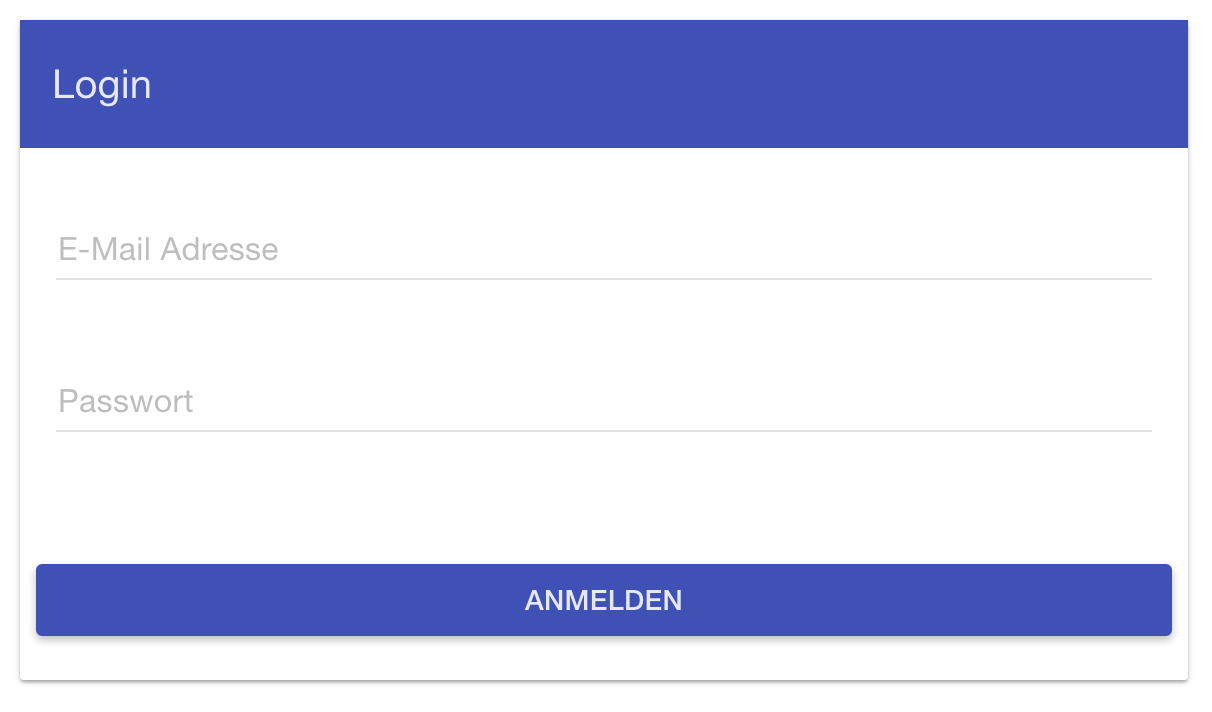
\includegraphics[width=0.5\textwidth]{images/frontend_login.png}
\caption{Anmeldeformular}
\label{frontend_login}
\end{figure}

\subsection{Hauptseite}
Die Hauptseite ist sehr schlicht aufgebaut und teilt sich auf in zwei Teile. 

\begin{figure}[H]
\centering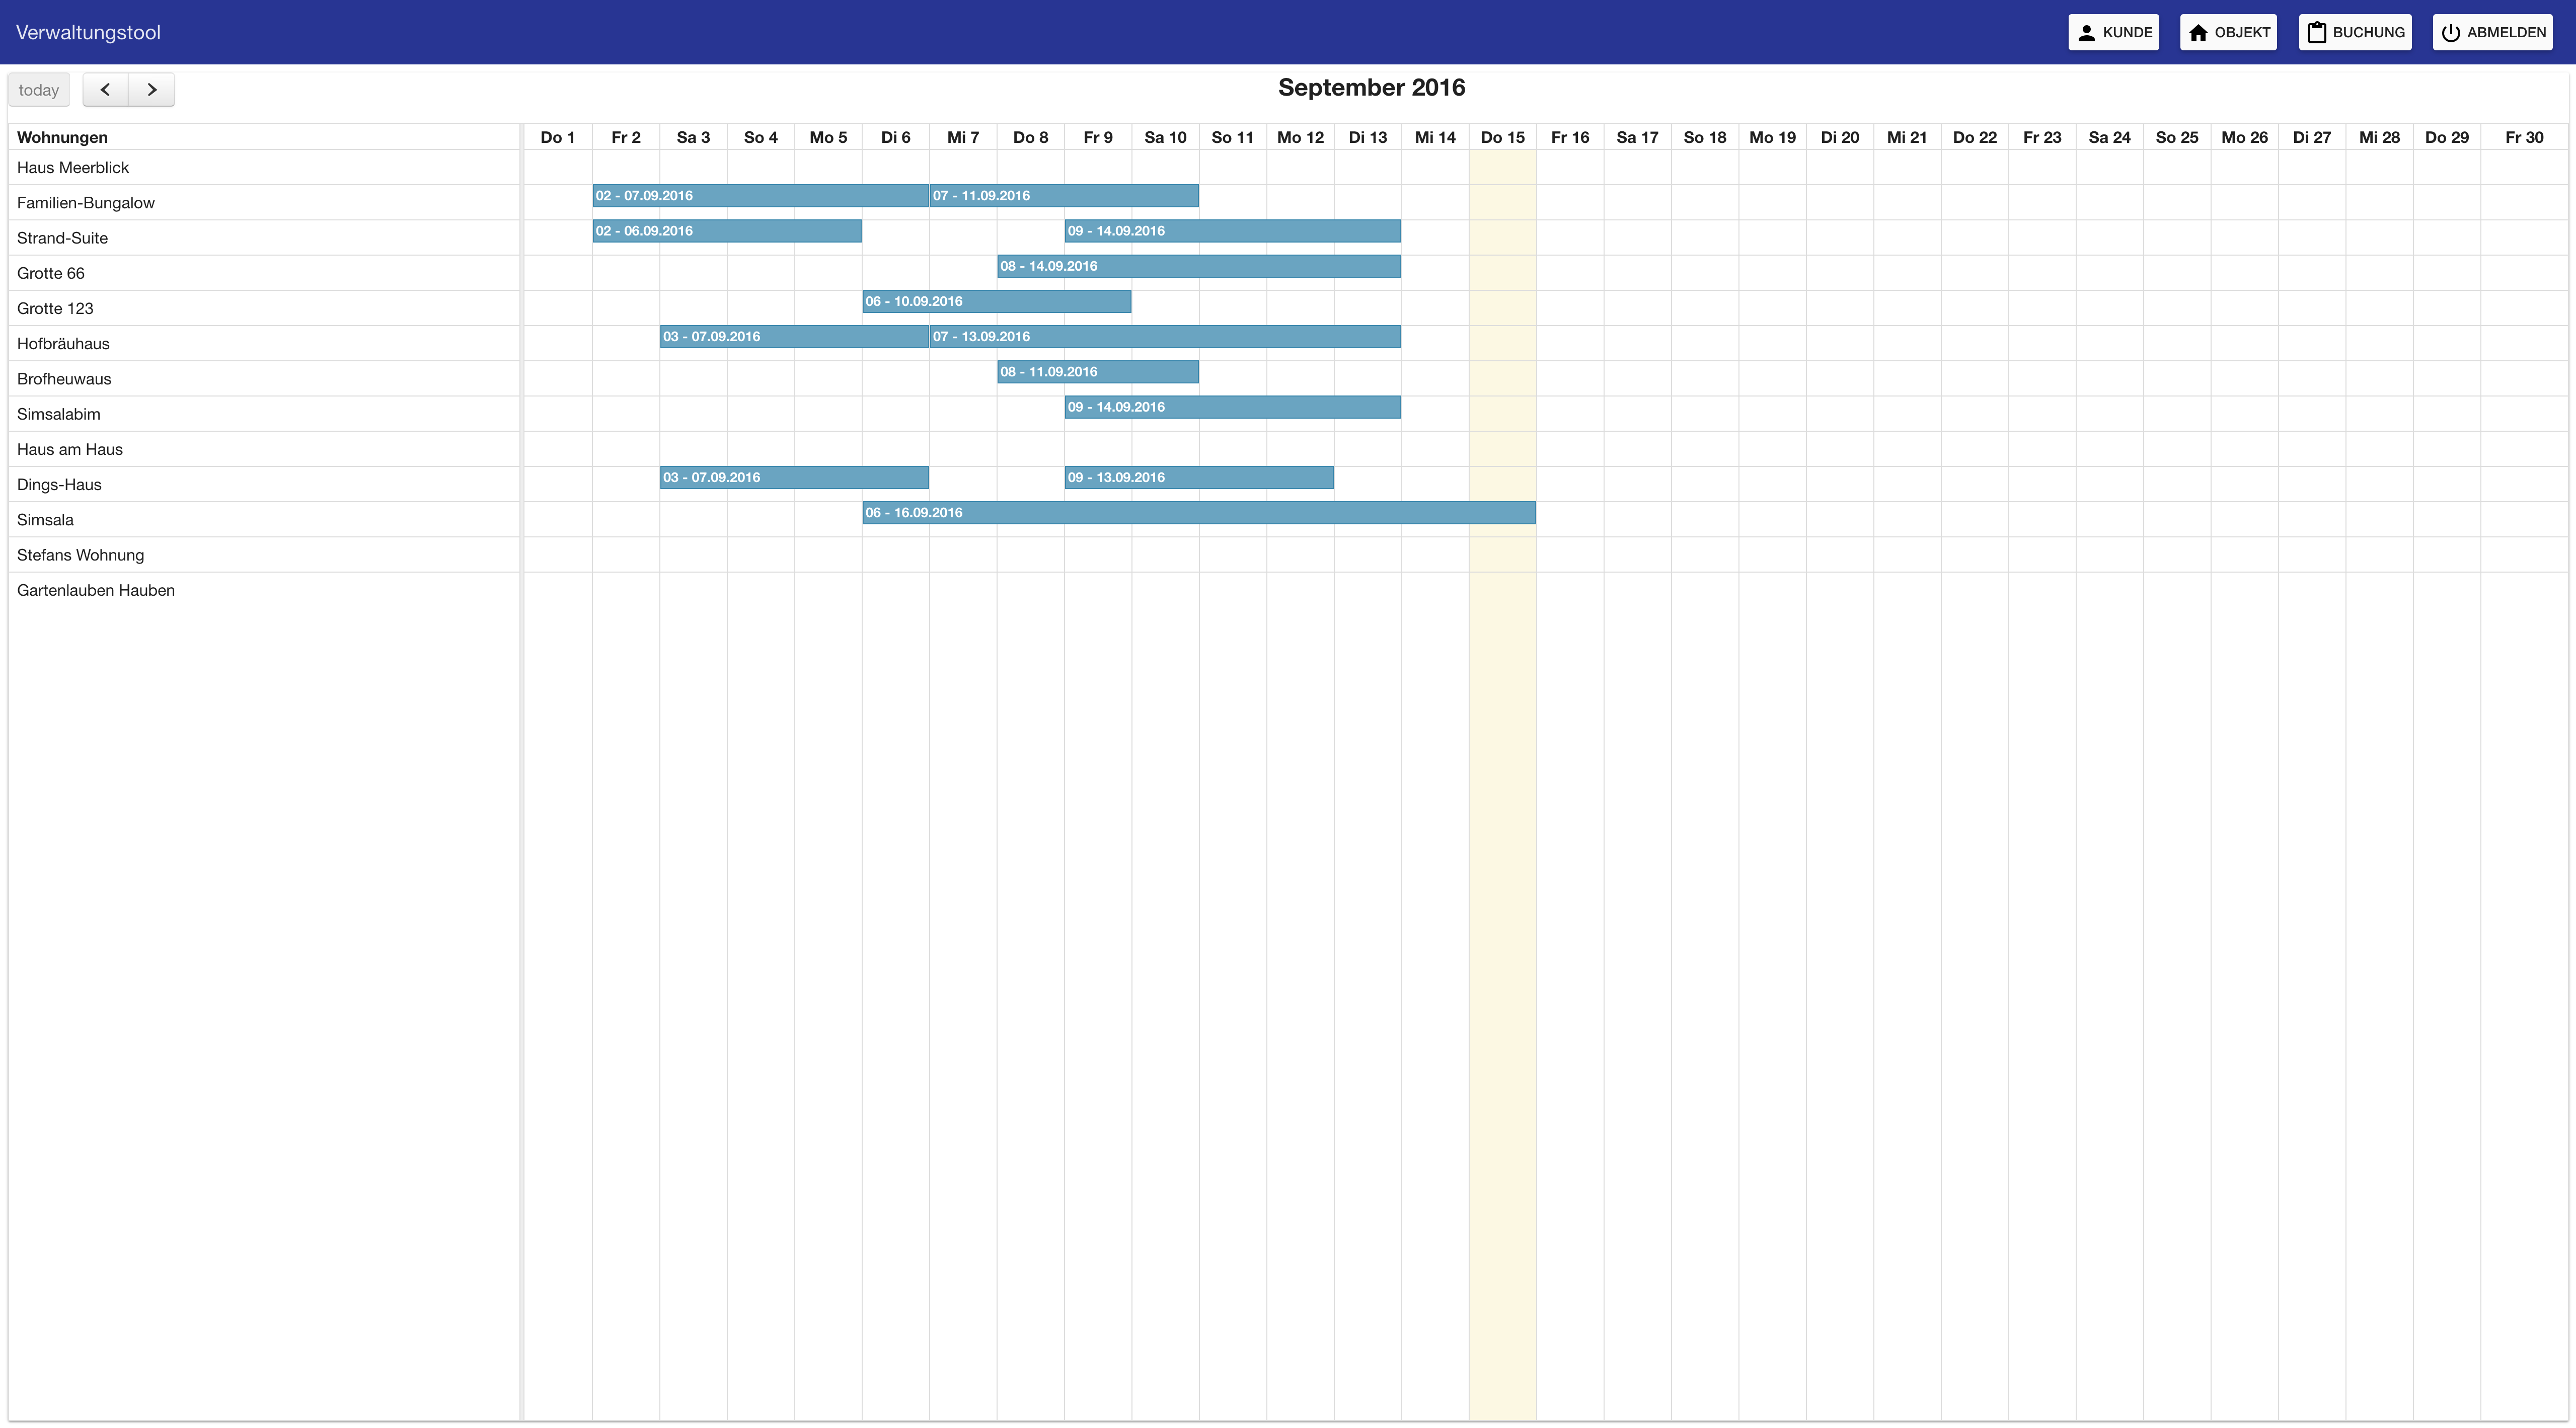
\includegraphics[width=1\textwidth]{images/frontend_mainpage.png}
\caption{Hauptseite}
\label{frontend_
mainpage}
\end{figure}

\subsubsection{Header}
Im Header befinden sich neben dem Programmlogo auch folgende vier Button:


\begin{description}
\item[Kunde]\hfill \\
Ein Dialog öffnet sich in dem Kunden hinzugefügt, bearbeitet oder gelöscht werden können.
\item[Objekt]\hfill \\ 
Ein Dialog öffnet sich in dem eine neue Ferienwohnung / Haus hinzugefügt werden kann. 
\item[Buchung]\hfill \\ 
Ein Dialog öffnet sich in dem eine neue Buchung hinzugefügt werden kann. 
\item[Logout]\hfill \\ 
Nach der Bestätigung eines Dialogs wird der Nutzer abgemeldet und auf die Login-Seite verwiesen. 
\end{description}

Sobald die Fenstergröße kleiner oder die Größe eines durchschnittlichen Tablets erreicht hat, werden die Buttons ausgeblendet. Stattdessen erscheint ein Symbol das bei Klick eine Seitennavigation einblendet in der sich alle Buttons befinden.

\begin{figure}[H]
    \centering
    \begin{minipage}[t]{0.49\linewidth}
        \centering
        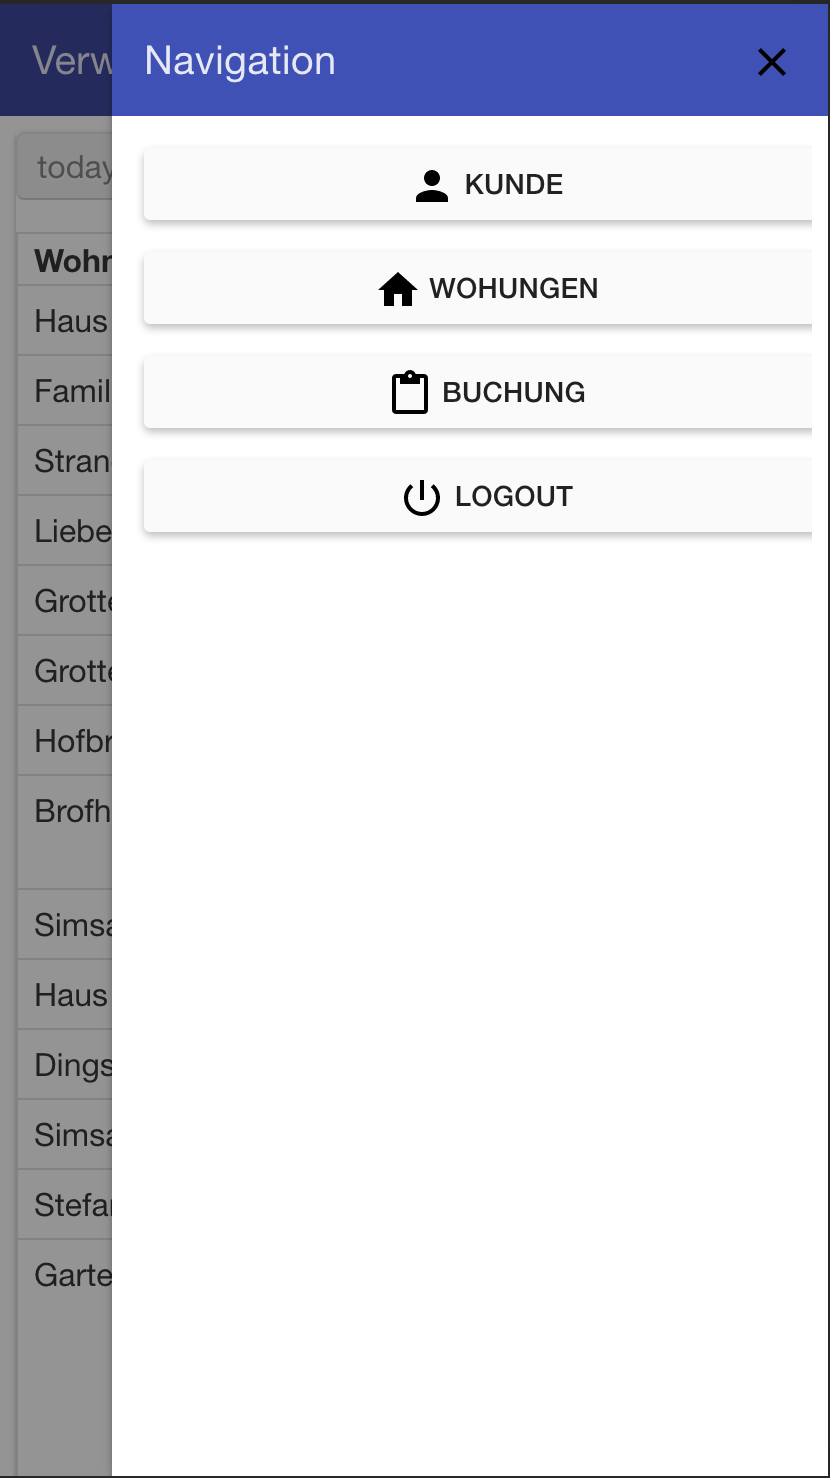
\includegraphics[width=\linewidth]{images/frontend_header_small.png}
        \label{frontend_header_small}
        \caption{Ansicht auf Mobilgeräten}
    \end{minipage}% <- sonst wird hier ein Leerzeichen eingefügt
    \hfill
    \begin{minipage}[t]{0.49\linewidth}
        \centering
        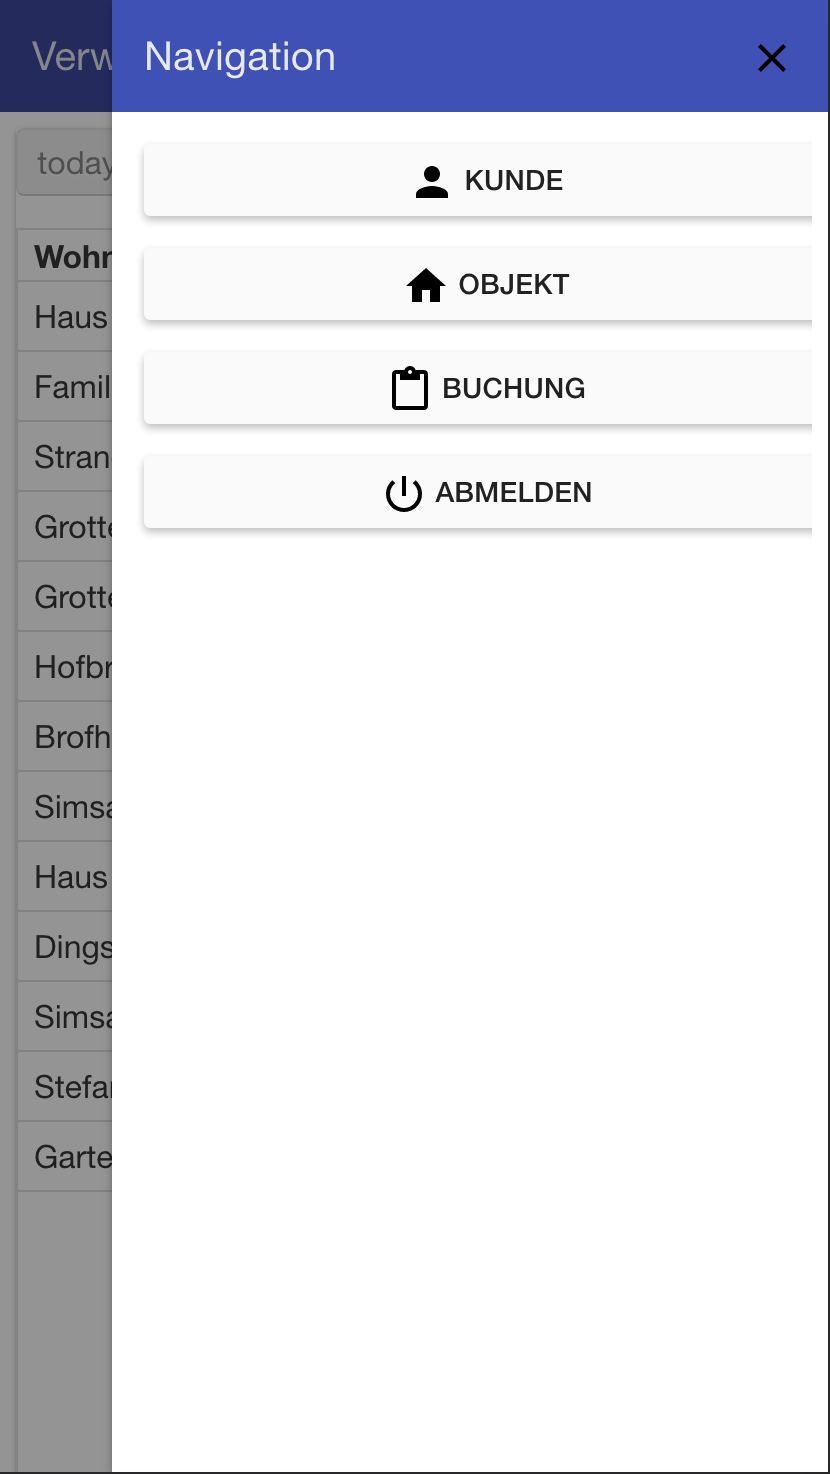
\includegraphics[width=\linewidth]{images/frontend_header_small_navigation.png}
        \label{frontend_header_small_navigation}
        \caption{Seitennavigation auf Mobil}
    \end{minipage}
\end{figure}


\subsubsection{Main}
In der Main befindet sich lediglich der Kalender, welcher auf voller Breite und Höhe abgebildet. 
Dieser ist aufgeteilt in folgende zwei Bereiche:
\begin{description}
\item[Objektübersicht]\hfill \\
Alle Objekte werden auf der linken Seite in form einer Liste dargestellt
\item[Buchungsübersicht]\hfill \\ 
Alle Tage des aktuellen Monats werden als Spalten angezeigt. Die Buchungen werden als Blöcke angezeigt und verbinden dessen Tage in Spalten.  
\end{description}

\subsection{Kunde}
Zusammen mit dem Objekt bildet der Kunde eine Buchung. Für die Kundeninformationen wurden alle Felder aus dem Projektzielen implementiert. Zudem sind alle Felder ausgenommen der Zusatzinformationen und der Firma Pflicht und werden beim Abschicken des Formulars überprüft, ob sie leer sind. Um die Eingabe des Geburtstages zu vereinfachen wurde ein für Tag, Monat und Jahr jeweils ein Dropdown-Menü bereitgestellt. Da das Mindestalter für Buchungen 18 Jahre ist, ist das höchste auszuwählende Jahr immer 18 Jahre vom aktuellen gerechnet. Das Datum wird im UNIX TIMESTAMP gespeichert. Sind alle Felder korrekt ausgefüllt, kann das Formular abgeschickt werden. Sobald die \texttt{submit} Funktion im Controller aufgerufen wird, werden alle Felder aus dem View einem \texttt{customer} JSON-Objekt gespeichert. Diese werden dem \texttt{Customer} Model übergeben und das Dialog geschlossen. 

Soll ein bestehender Kunde bearbeitet werden muss dieser zunächst über das Suchfeld gesucht werden. Mittels des Lupensymbol im Kopfbereich des Dialog wird die Suchleiste ein oder ausgeblendet. Sobald das Suchfeld fokussiert wird, wird eine Funktion im Controller angestoßen welche alle Kunden mit Vor und Nachname als Auswahlmöglichkeit auflistet. Dafür wird die Liste aller Kunden im Model angefordert. Dieses Liefert ein Array mit allen Kundenobjekten. Bei einer hohen Anzahl an Kunden kann sich die Suche schwierig gestalten. Aus diesem Grund kann der Kunde durch eintippen von Buchstaben gefiltert werden. Jeder weitere Buchstabe schränkt die Suche nach dem Vornamen ein und es werden nur Kunden angezeigt dessen Nachname die eingegebene Zeichenkette beinhalten. 

\begin{figure}[H]
\centering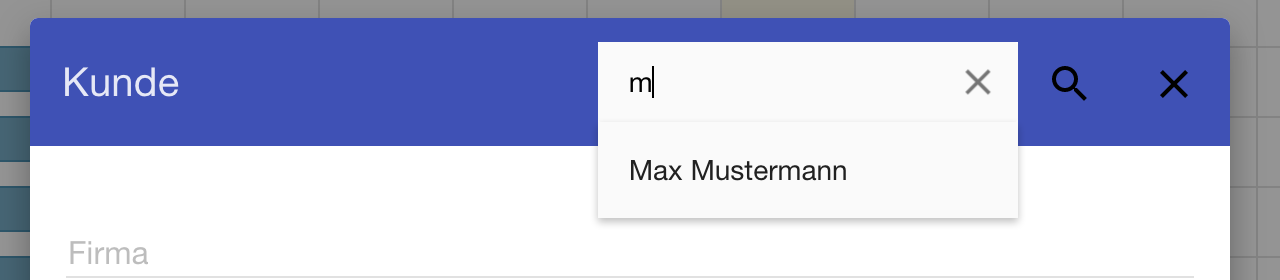
\includegraphics[width=0.5\textwidth]{images/frontend_customer_search.png}
\caption{Kundensuche}
\label{customer_search}
\end{figure}

\begin{figure}[H]
    \centering
    \begin{minipage}[t]{0.49\linewidth}
        \centering
        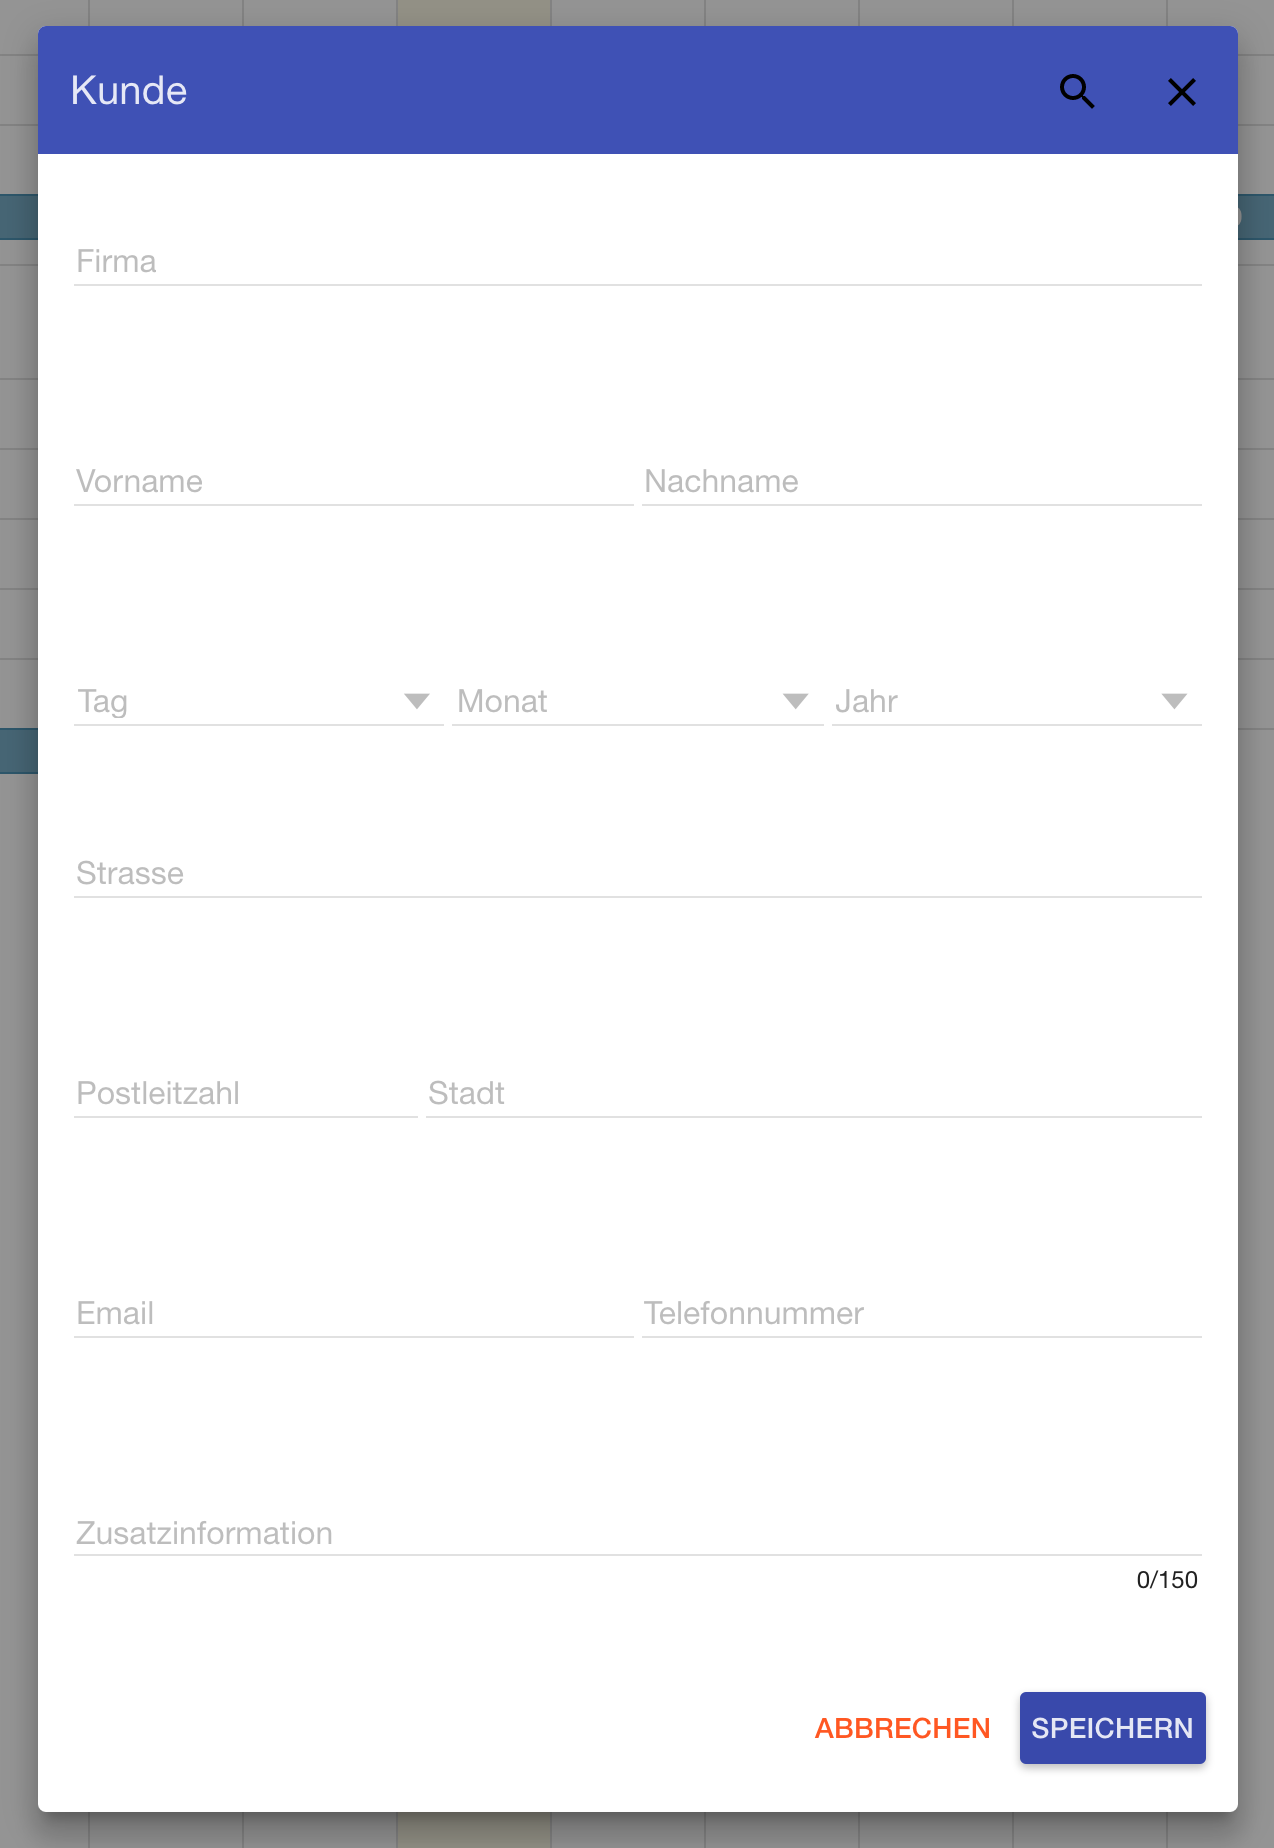
\includegraphics[width=\linewidth]{images/frontend_customer_new.png}
        \label{frontend_customer_new}
        \caption{Neuen Kunden erstellen}
    \end{minipage}% <- sonst wird hier ein Leerzeichen eingefügt
    \hfill
    \begin{minipage}[t]{0.49\linewidth}
        \centering
        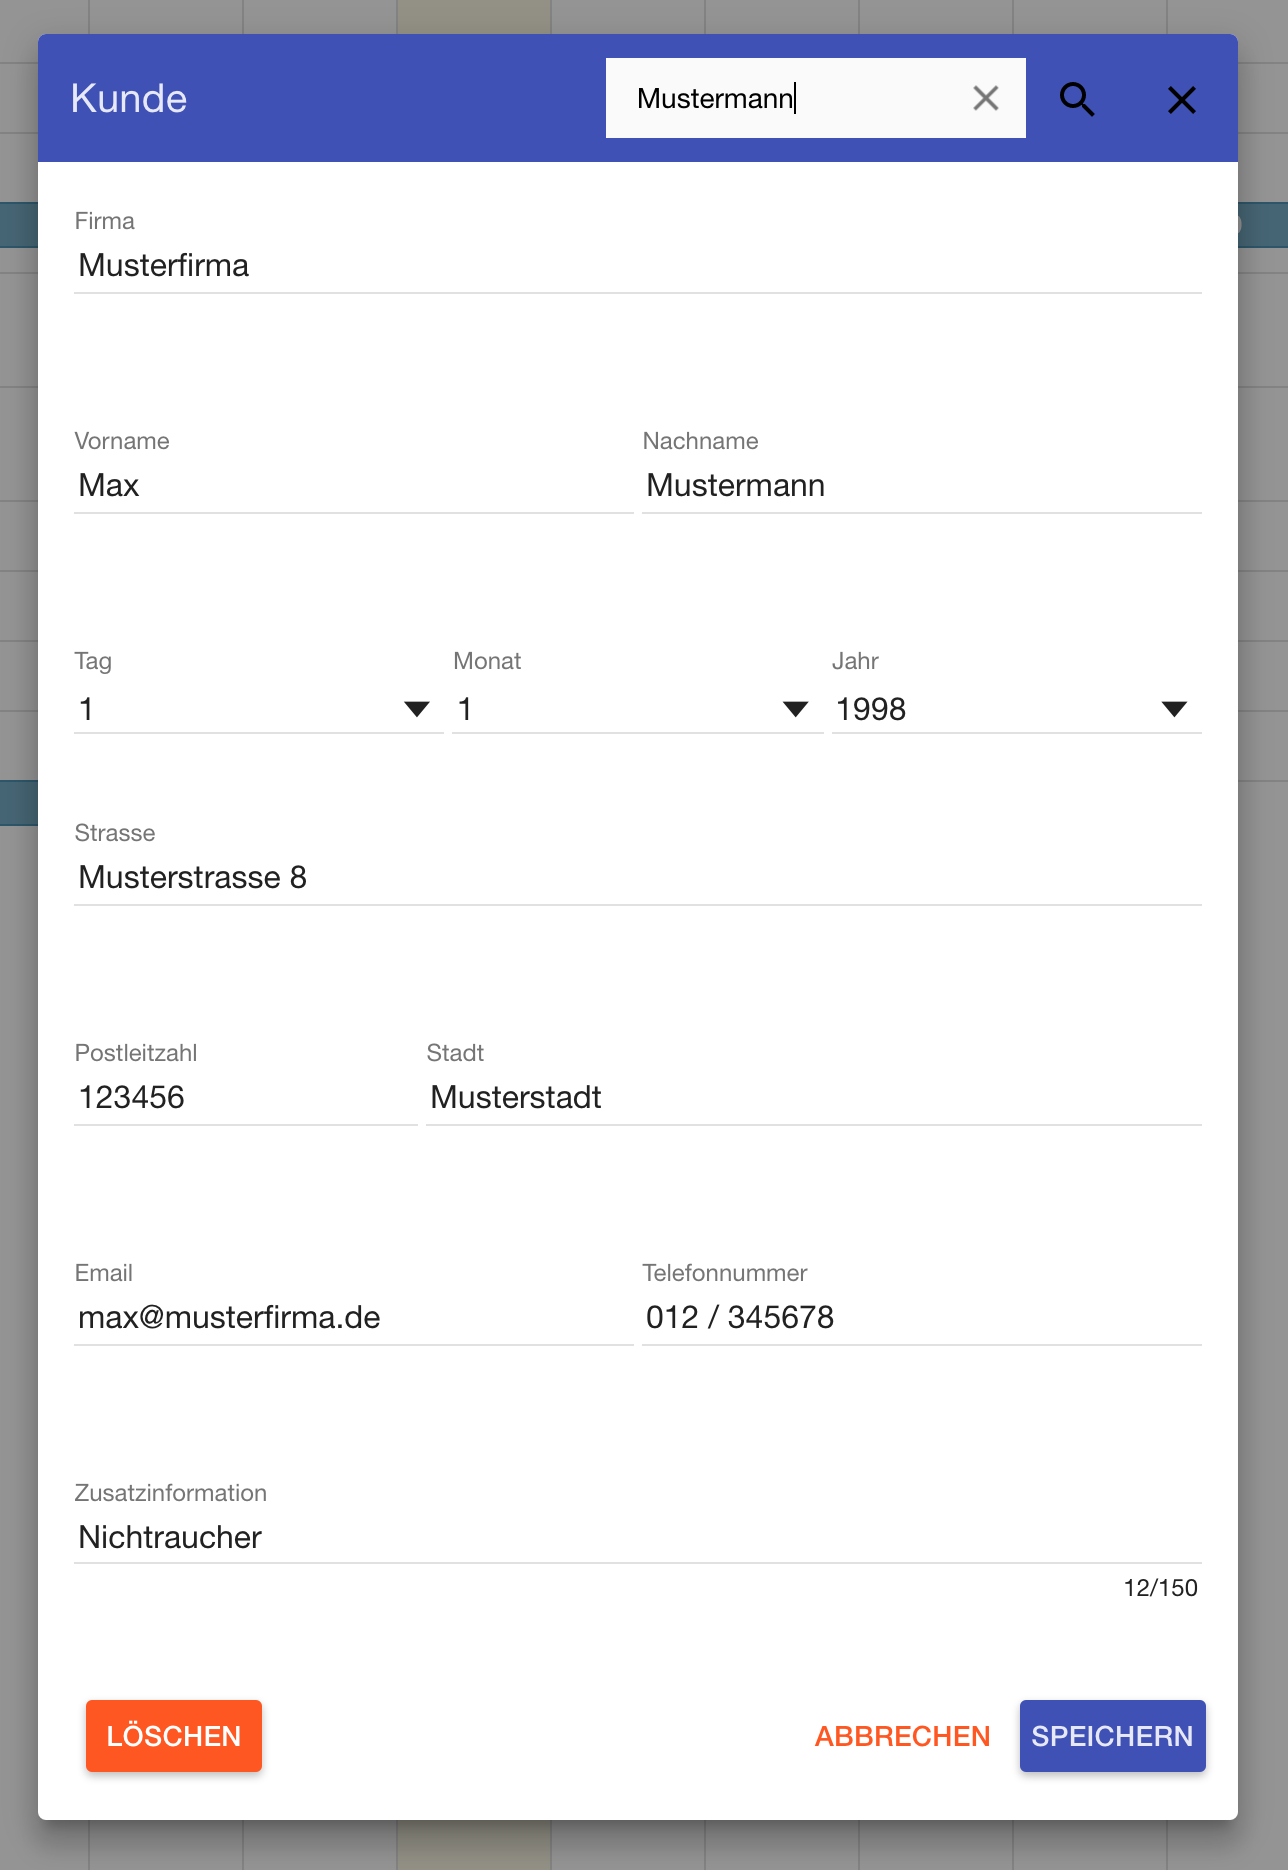
\includegraphics[width=\linewidth]{images/frontend_customer_edit.png}
        \label{frontend_customer_edit}
        \caption{Kunden bearbeiten}
    \end{minipage}
\end{figure}

Wurde ein Kunde ausgewählt, werden alle Daten aus dem JSON-Objekt ausgelesen und in die Input Felder eingefügt. Gleichzeitig wird ein Button angezeigt der das Löschen eines Kunden aus der Datenbank ermöglicht. Um einem Fehler vorzubeugen muss zusätzlich noch ein Dialog bestätigt werden. Wird dieser bestätigt übergibt der Controller dem Model die UUID des Kunden in einer \texttt{delete} Funktion. 
%TODO delete customer in model

Wenn Daten verändert wurden, können diese wie auch beim Hinzufügen eines neuen Kunden bestätigt werden. Dabei wird die selbe Funktion aufgerufen. In diesem Fall wird im Controller die \texttt{upsert} Funktion im Model aufgerufen. Je nachdem, ob es sich dabei um einen bestehenden Eintrag in der Datenbank handelt oder der Eintrag bereits vorhanden ist wird ein \texttt{Update} oder \texttt{Insert} durchgeführt. Dafür ist die von der Datenbank vergebene UUID ausschlaggebend.

Soll weder ein neuer Kunde hinzugefügt noch ein bestehender bearbeitet werden kann das Dialog über den \grqq Abbrechen\glqq Button, das \grqq X\glqq oder einen Klick ausserhalb des Dialogs geschlossen werden. Für den Controller ist das ein und die selbe Funktion. Dieser ruft lediglich die \texttt{hide} Methode des Dialogs auf und das Dialogfenster wird ausgeblendet. Dabei werden auch alle Daten aus den Feldern entfernt.





\subsection{Objekt}
Als Objekt wird eine Ferienwohnung oder Haus bezeichnet. Wie auch beim Kunden können Objekte verschiedene Informationen gespeichert werden. Die beiden gewünschten Felder aus den Projektzielen wurden übernommen. Dazu gehört die Eingabe des Namens in ein Textfeld. Wird das Feld fokussiert und ohne Eingabe verlassen erscheint eine Fehlermeldung mit dem Hinweis das Feld auszufüllen. Wird dieser Hinweis ignoriert und der Nutzer versucht das Formular abzuschicken, überprüft der View, ob alle als Pflicht gekennzeichneten Felder ausgefüllt wurden und der \texttt{submit} Button gedrückt wurde. Ist eines dieser Angaben \texttt{false} wird das Formular erst gar nicht abgeschickt.

\begin{figure}[H]
    \centering
    \begin{minipage}[t]{0.49\linewidth}
        \centering
        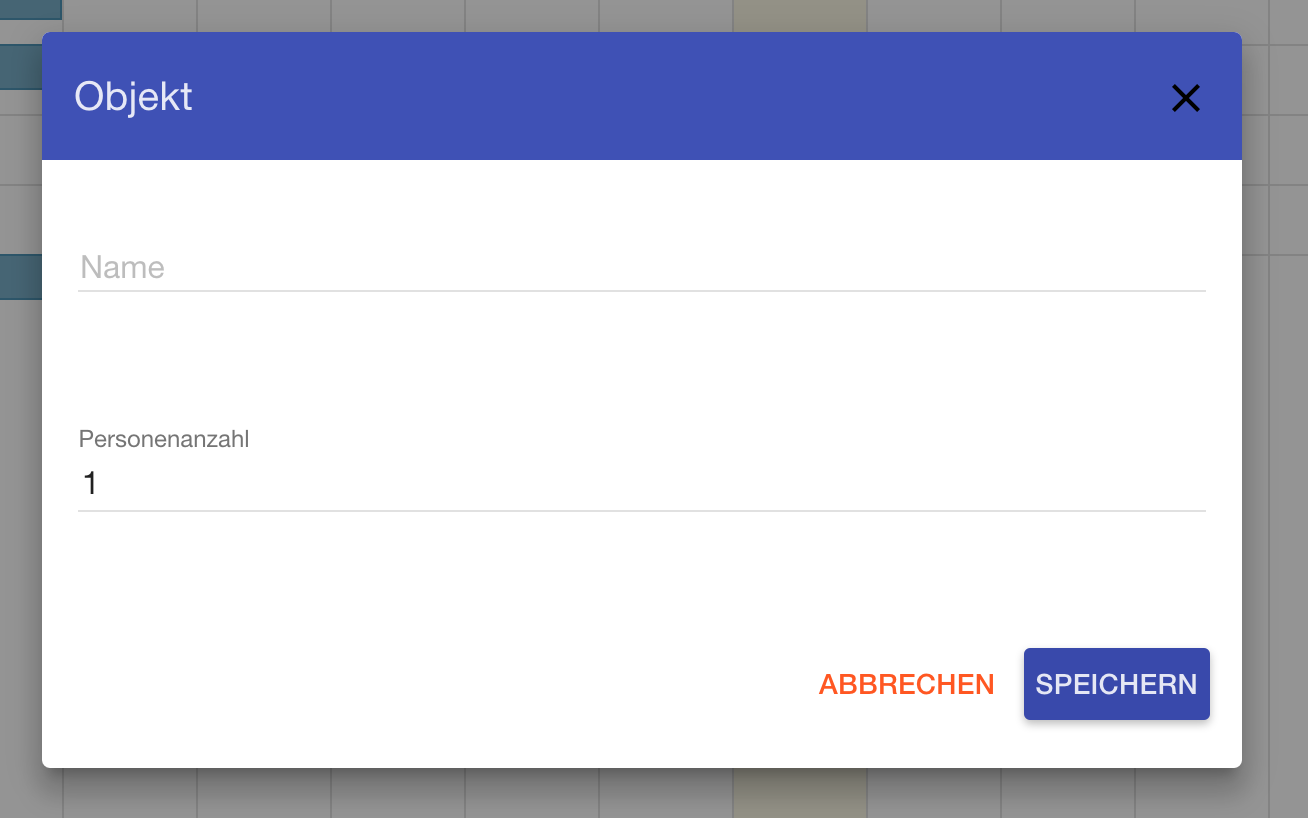
\includegraphics[width=\linewidth]{images/frontend_resource_new.png}
        \label{frontend_resource_new}
        \caption{Objekt erstellen}
    \end{minipage}% <- sonst wird hier ein Leerzeichen eingefügt
    \hfill
    \begin{minipage}[t]{0.49\linewidth}
        \centering
        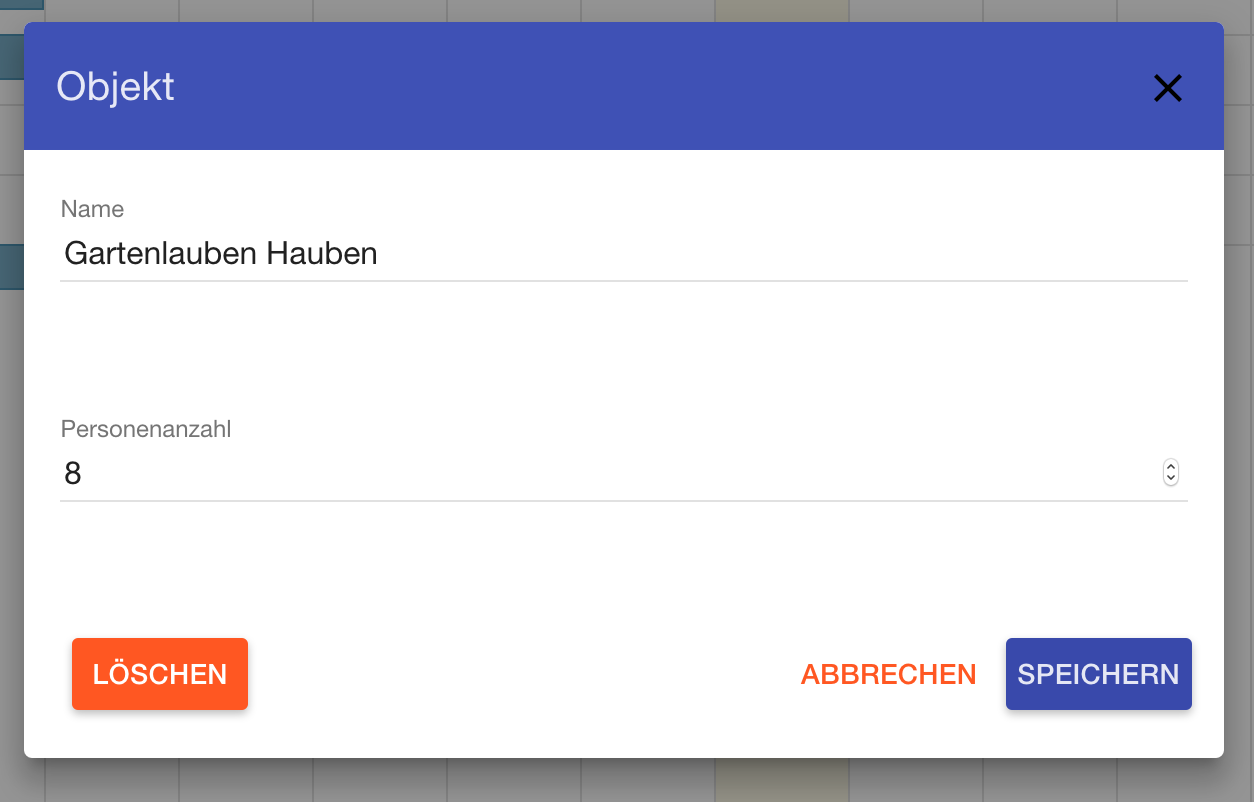
\includegraphics[width=\linewidth]{images/frontend_resource_edit.png}
        \label{frontend_resource_edit}
        \caption{Objekt bearbeiten}
    \end{minipage}
\end{figure}

\begin{figure}[H]
\centering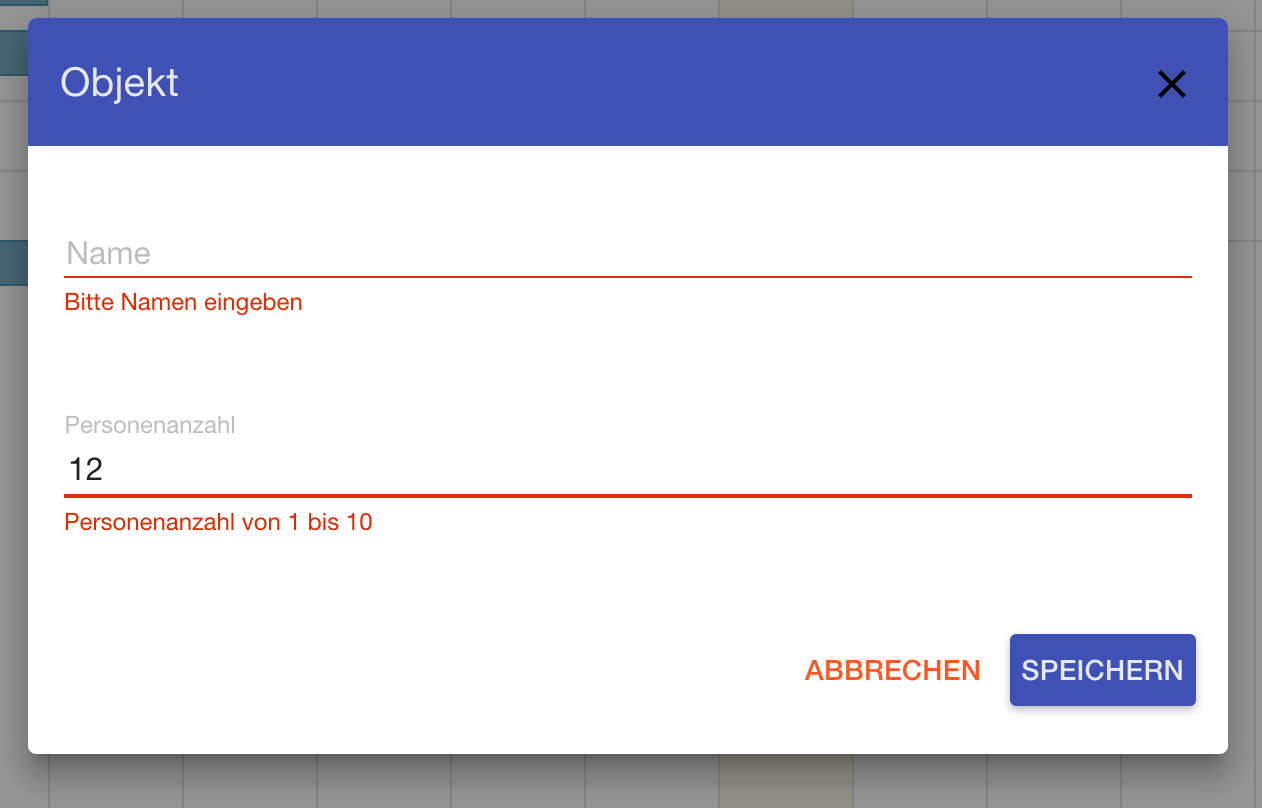
\includegraphics[width=0.5\textwidth]{images/frontend_resource_fail.png}
\caption{Löschen Bestätigungsdialog}
\label{frontend_resource_fail}
\end{figure}

 Auch bei der Angabe der maximalen Personenanzahl wurde darauf geachtet Falscheingaben abzufangen. Standardmäßig ist das minimum von 1 eingestellt. Der Nutzer hat die Möglichkeit mit Hilfe von Pfeilen den Wert zu Verändern. Die Maximale Anzahl von Personen ist 10 für jedes Objekt. Da es auch möglich ist Manuell eine Zahl einzugeben, wird ebenfalls überprüft, ob sich die Zahl in der Range zwischen 1 und 10 befindet. Ist dies nicht der Fall wird ein Hinweis ausgegeben und das Formular kann nicht abgeschickt werden. Sind alle Angaben korrekt und der \texttt{submit} Button wird betätigt wird das Formular abgeschickt. Im Controller wird eine Funktion aufgerufen in der die Daten aus den Feldern in ein JSON-Objekt gespeichert werden. Dieses wird der \texttt{upsert} Methode des Models übergeben. 

Um ein bereits existierendes Objekt bearbeiten zu können muss dies anders als bei den Kunden in der Auflistung in der main ausgewählt werden. Auch hier werden die Daten anhand der UUID aus der Datenbank geladen und in die Felder eingefügt. Zusätzlich wird der Button zum Löschen des Objektes angezeigt. Die Besonderheit bei der Änderung von Daten ist eine Eigenschaft im JSON-Objekt in dem die Informationen der Felder gespeichert werden. Neben des Namens und der Personenanzahl wird die ID des Objektes gespeichert. Ist, wie bei einer Änderung, bereits eine UUID vorhanden, wird diese als Wert gespeichert. Wird eine Objekt neu hinzugefügt ist der Wert \texttt{undefined}. Diese Information erlaubt wird in der \texttt{upsert} Methode des Models abgefragt und dementsprechend ein neues Objekt hinzugefügt oder ein bestehendes aktualisiert.
%TODO how works upsert at model

  
\subsection{Buchung}
Eine Buchung ist ein Zusammenschluss aus Kunde, Objekt, Personenanzahl, Startdatum und Enddatum. Wie bei der Bearbeitung von Kunden, kann der Nutzer den Kunden über ein Suchfeld filtern und Auswählen. Zusätzlich funktioniert das ebenfalls für das Objekt. 
%TODO load data from model
Wenn eine neue Buchung hinzugefügt wird, wird zunächst die Auswahl der Personenanzahl ausgeblendet. Erst wenn ein Objekt im Suchfeld ausgewählt wurde, wird die Auswahl in form eines Dropdown-Menüs im View angezeigt. Im Controller wird vorher die maximale Personenanzahl des ausgewählten Objektes aus dem JSON-Objekt entnommen und somit die zur Auswahl stehenden Zahlen ermittelt. So zeigt das Dropdown-Menü nur genau die Anzahl von Personen an die dieses Objekt zur verfügung stellt. Für das Startdatum und Enddatum wurden, anders als beim Kunden, ein Datepicker zur verfügung gestellt, der es dem Nutzer erlaubt das Datum durch einfache Auswahl in einem Kalender festzulegen. Standardmäßig ist das aktuelle Datum eingestellt.

\begin{figure}[H]
    \centering
    \begin{minipage}[t]{0.49\linewidth}
        \centering
        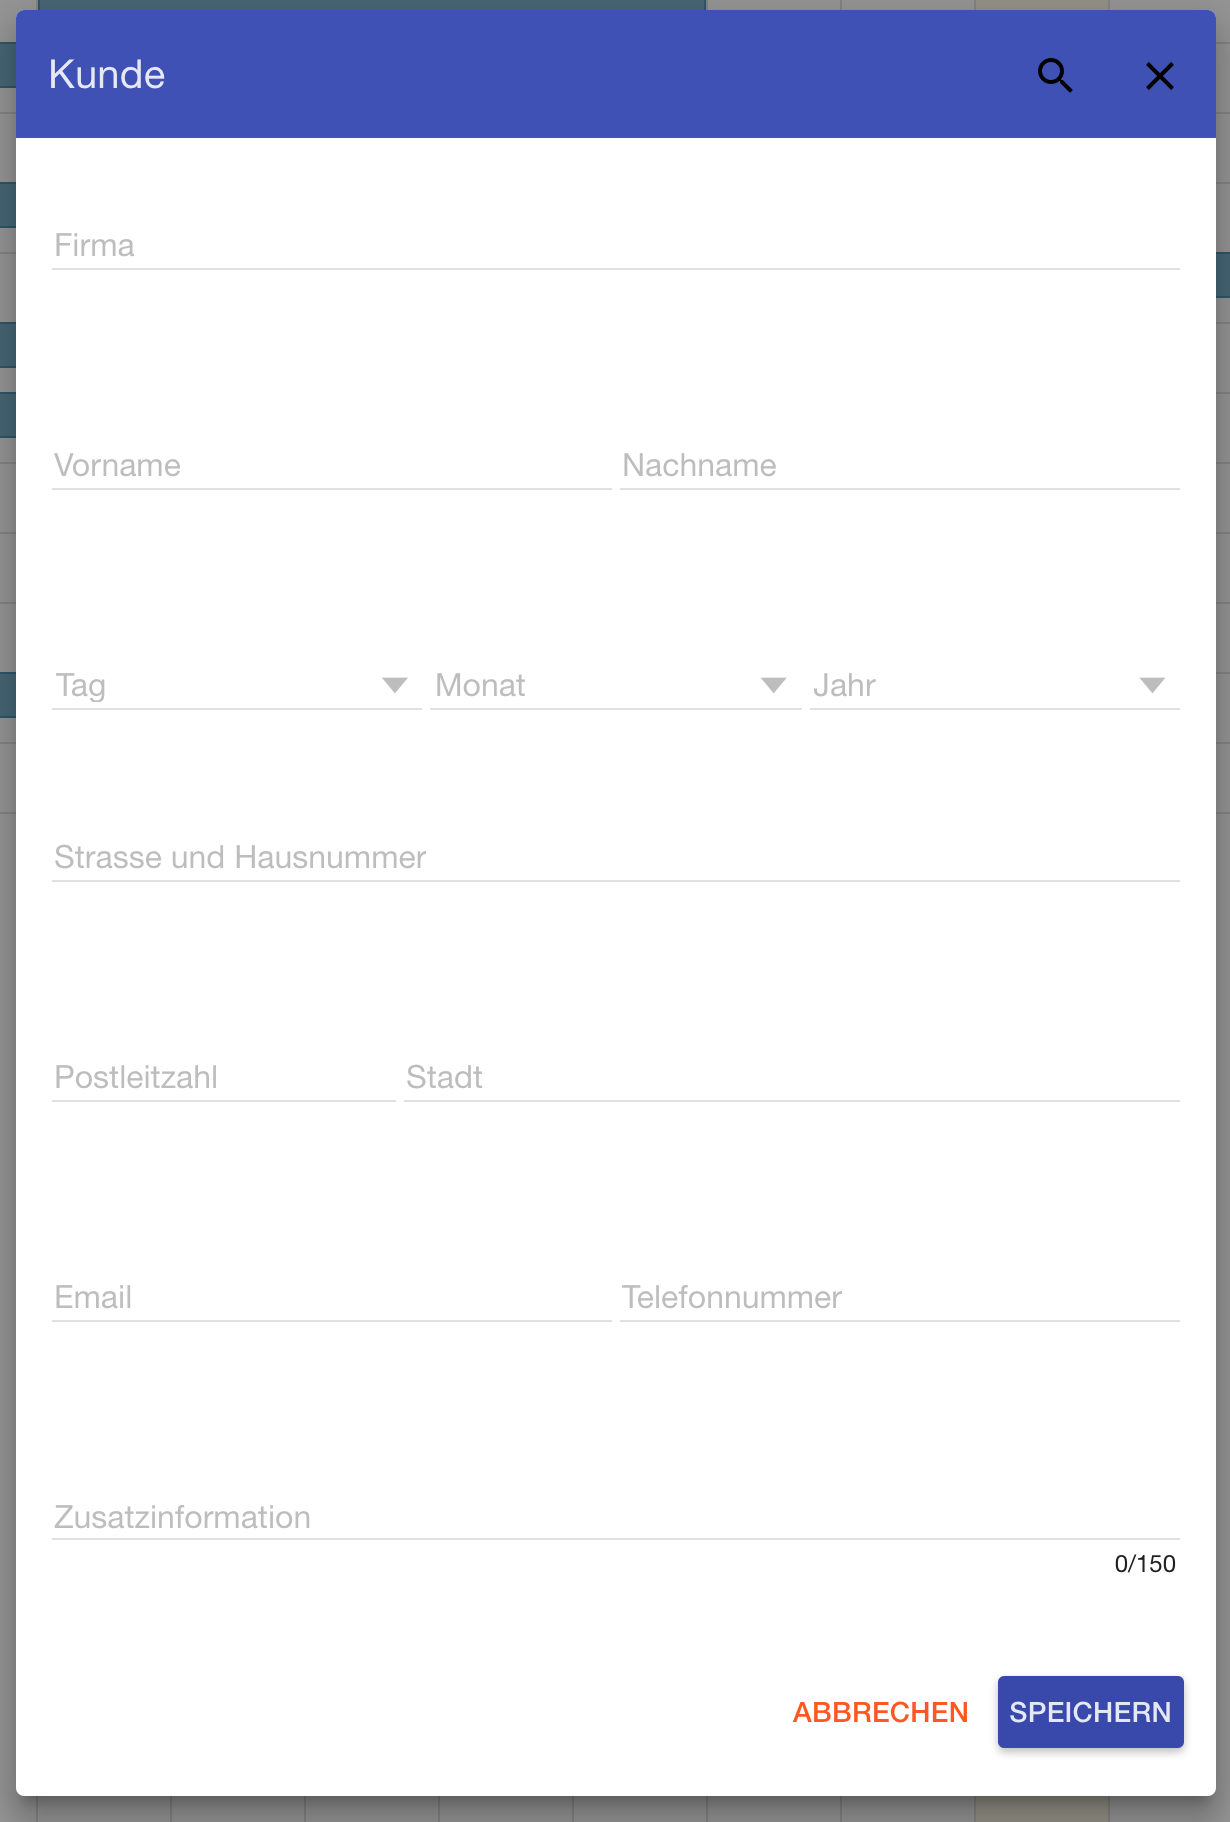
\includegraphics[width=\linewidth]{images/frontend_booking_new.png}
        \label{frontend_booking_new}
        \caption{Objekt erstellen}
    \end{minipage}% <- sonst wird hier ein Leerzeichen eingefügt
    \hfill
    \begin{minipage}[t]{0.49\linewidth}
        \centering
        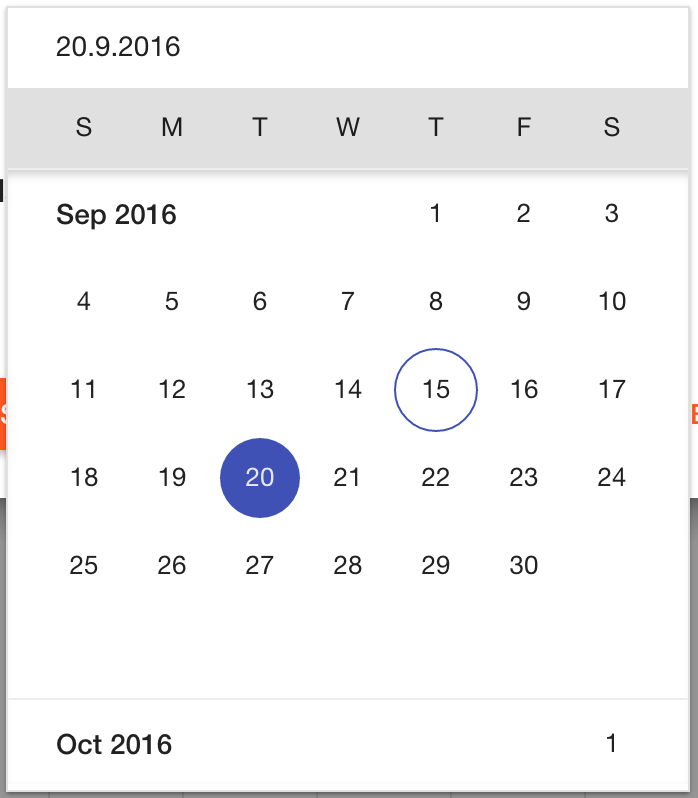
\includegraphics[width=\linewidth]{images/frontend_booking_calender.png}
        \label{frontend_booking_calender}
        \caption{Objekt Fehlereingabe}
    \end{minipage}
\end{figure}

Um eine Buchung bearbeiten zu können muss diese anders als beim Kunden oder Objekt zunächst in der Buchungsübersicht gesucht werden. Wurde die passende Buchung gefunden und ausgewählt, öffnet sich das Modal mit den hinterlegten Daten. Hier wird die Personenauswahl angezeigt und mit dem eingetragenem Wert vordefiniert. Auch hier besteht die Möglichkeit durch den angezeigten Löschen-Button die Buchung aus der Datenbank zu entfernen.  

\begin{figure}[H]
    \centering
    \begin{minipage}[t]{0.49\linewidth}
        \centering
        
\includegraphics[width=\linewidth]{images/frontend_booking_delete_dialog.png}
        \label{frontend_booking_delete_dialog}
        \caption{Objekt erstellen}
    \end{minipage}% <- sonst wird hier ein Leerzeichen eingefügt
    \hfill
    \begin{minipage}[t]{0.49\linewidth}
        \centering
        
\includegraphics[width=\linewidth]{images/frontend_toast.png}
        \label{frontend_toast}
        \caption{Objekt Fehlereingabe}
    \end{minipage}
\end{figure}


Wird ein Dialog bestätigt wird erscheint für drei Sekunden am oberen rechten Fensterrand ein Nachricht. Ein sogenannter Toast fährt herunter und zeigt die Erfolgsmeldung und einen Button zum schließen an. In der mobilen Ansicht fährt der Dialog, in voller Bildschirmbreite, von unten herein. 

\subsection{Kalender}

%TODO write text about the main calender
 
\section{Backend}

\chapter{Frontend}
In diesem Kapitel wird die prototypische Entwicklung des Frontend beschrieben. Dabei werden anhand der verschiedenen Bereiche die Umsetzung der Projektstruktur und die Funktionsweise des Programmes erläutert.

\section{Login}
Da die Software, wie in den Projektzielen erwähnt, nicht nur intern im Büro sondern auch von extern aus erreichbar sein muss, ist es nötig eine Authentifizierung einzurichten damit unbefugte keine Möglichkeiten haben die Daten zu verändern oder einzusehen. Um die Software nutzen zu können, benötigt der Bearbeiter eine gültige Kombination aus E-Mail und Passwort. Schon bei der Eingabe der Daten wird überprüft, ob die Felder leer sind oder es sich überhaupt um eine E-Mail handelt. Dabei wird abgefragt, ob ein (at)-Zeichen vorhanden ist und darauf ein Punkt folgt.

Sobald das Formular abgeschickt wurde, werden die Daten zunächst im \texttt{login.js} Controller entgegengenommen. Von da aus werden diese an den Authenticate-Service weitergegeben um sie von da aus an das Backend weiter zu reichen. In Firebase werden sie dann mit den hinterlegten Daten verglichen. Sind E-Mail und Passwort nicht korrekt oder nicht vorhanden, wird eine Fehlermeldung zurückgegeben die der Controller im View anzeigt. Sofern alle Angaben korrekt sind, wird der Nutzer weiter zu der Hauptseite geleitet. 

Da es sich hierbei um eine Betriebsinterne Software handelt, wird eine Registrierung nicht benötigt. Die Emailadresse und das Passwort werden Manuell im Backend hinzugefügt, bearbeitet oder entfernt. 
Die Folgende Abbildung \ref{frontend_login} zeigt, wie der Anmeldebildschirm aussieht. 

\begin{figure}[H]
\centering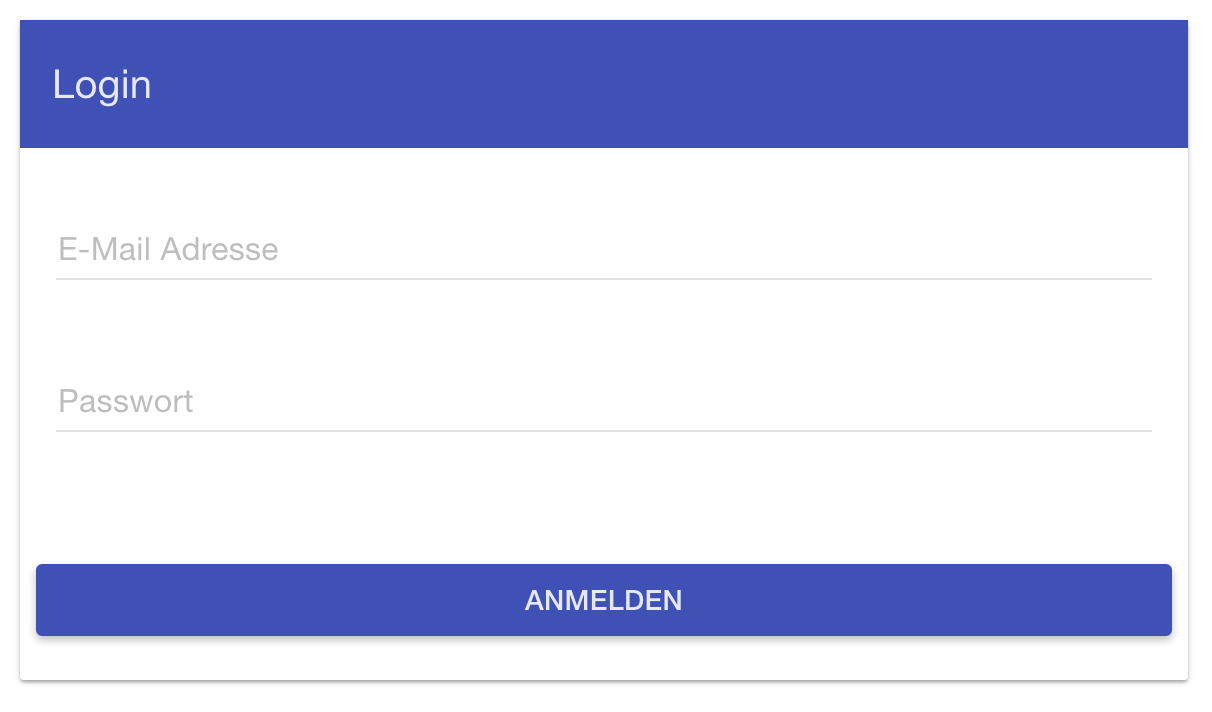
\includegraphics[width=0.5\textwidth]{images/frontend_login.png}
\caption{Anmeldeformular}
\label{frontend_login}
\end{figure}

\section{Hauptseite}
Aus den in den Projektzielen gesteckten Bedingungen ergibt sich in Abbildung \ref{frontend_mainpage} gezeigte Hauptseite. Diese ist schlicht aufgebaut bietet jedoch gleichzeitig alle gewünschten Funktionen, die mit einem Klick erreicht werden können.

\begin{figure}[H]
\centering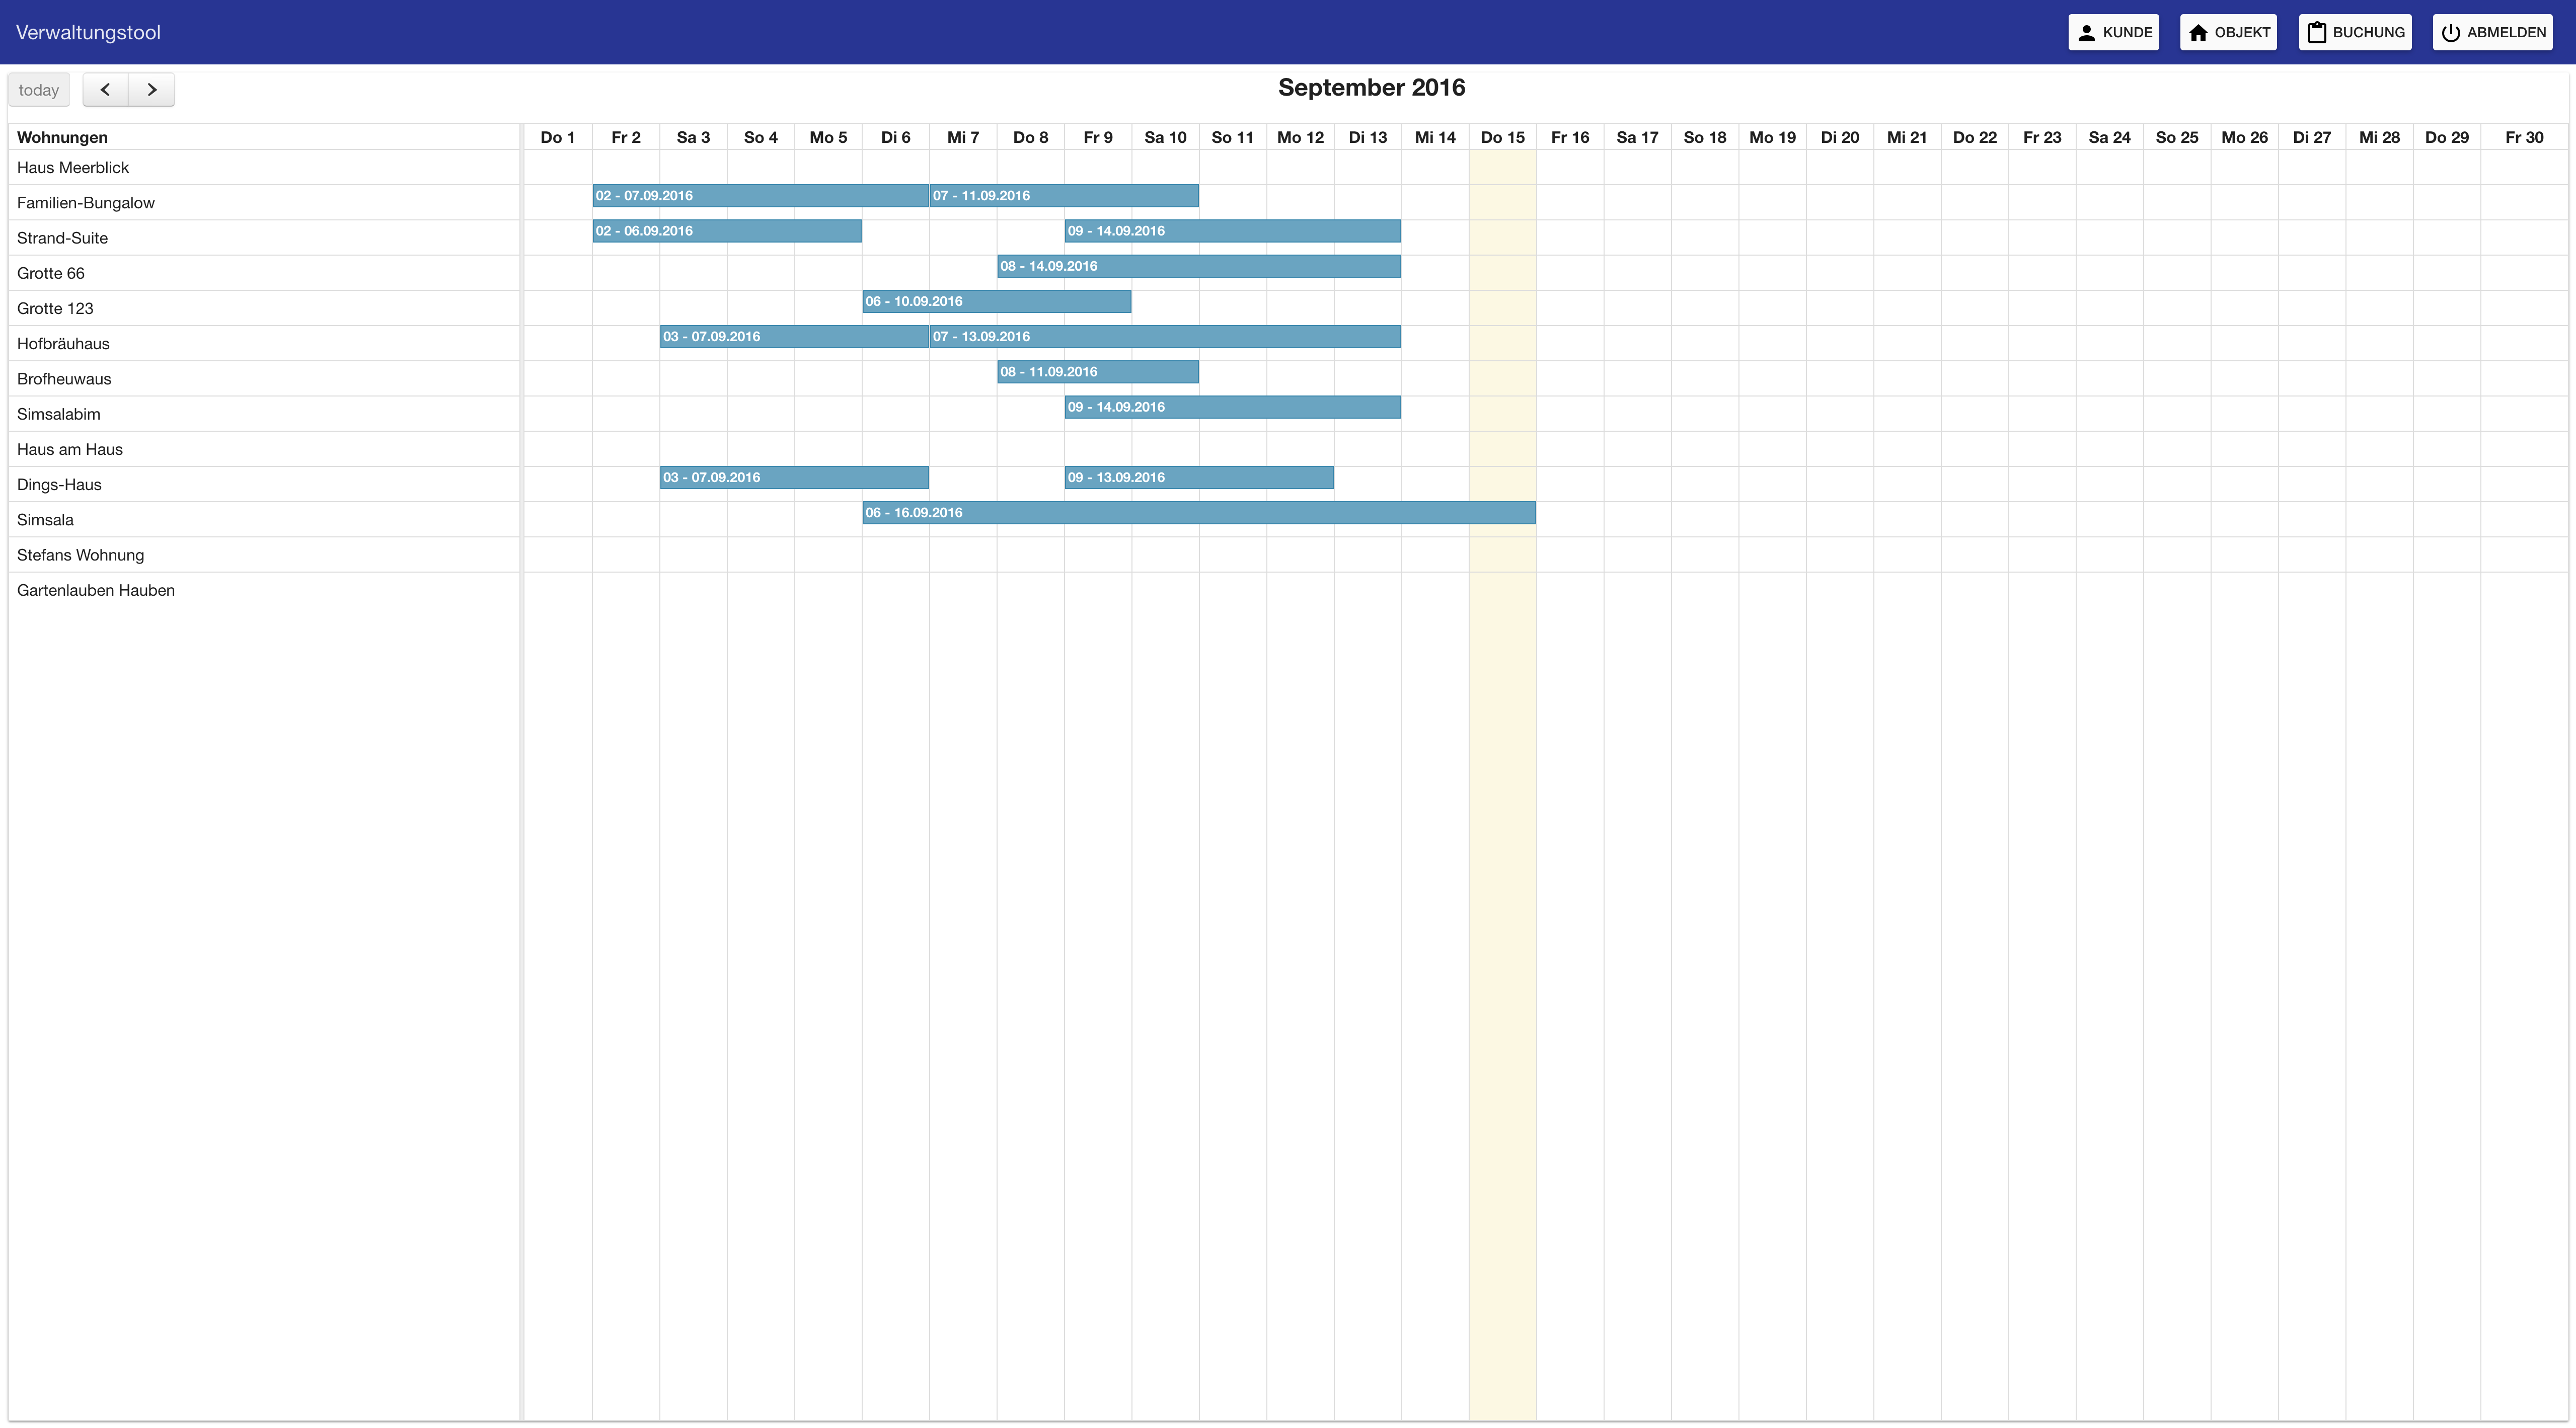
\includegraphics[width=1\textwidth]{images/frontend_mainpage.png}
\caption{Hauptseite}
\label{frontend_mainpage}
\end{figure}

\subsection{Header}
Im Kopfbereich befinden sich neben dem Programmname auch folgende vier Button:

\begin{description}
\item[Kunde]\hfill \\
Ein Dialog öffnet sich in dem Kunden hinzugefügt werden können. Nach einer Suche ist das Bearbeitung und Löschen ebenfalls möglich.
\item[Objekt]\hfill \\ 
Ein Dialog öffnet sich in dem eine neue Ferienwohnung / Haus hinzugefügt werden kann. 
\item[Buchung]\hfill \\ 
Ein Dialog öffnet sich in dem eine neue Buchung hinzugefügt werden kann. 
\item[Logout]\hfill \\ 
Nach der Bestätigung eines Dialogs wird der Nutzer abgemeldet und auf die Login-Seite verwiesen. 
\end{description}

Sobald die Fenstergröße kleiner ist oder die Größe eines durchschnittlichen Tablets erreicht wurde, werden die Buttons im Kopfbereich ausgeblendet (Abbildung \ref{frontend_header_small}). Stattdessen erscheint ein Symbol das bei Klick eine Seitennavigation einblendet in der sich alle Buttons befinden (Abbildung \ref{frontend_header_small_navigation}).

\begin{figure}[H]
    \centering
    \begin{minipage}[t]{0.49\linewidth}
        \centering
        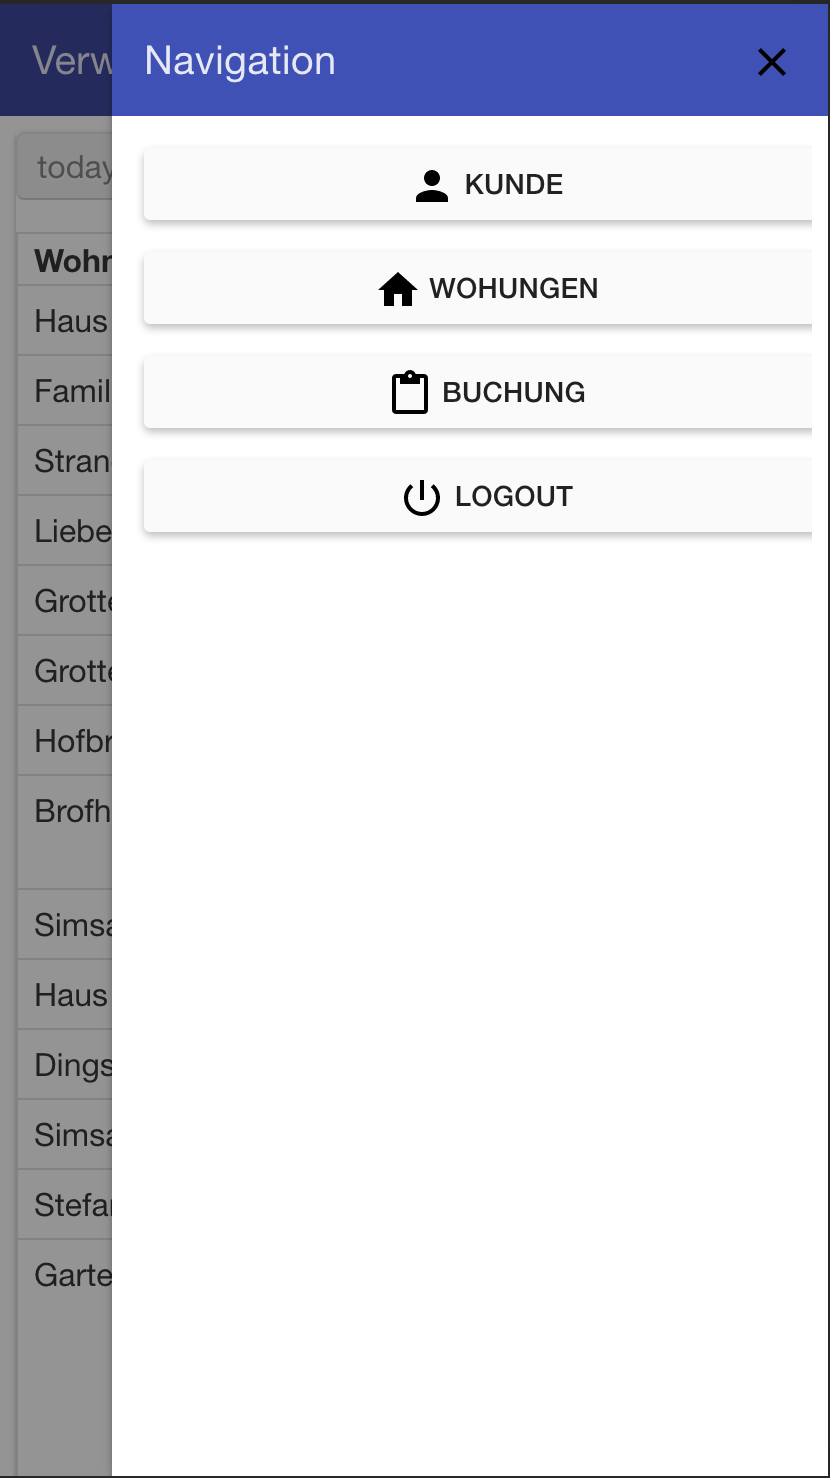
\includegraphics[width=\linewidth]{images/frontend_header_small.png}
        \label{frontend_header_small}
        \caption{Ansicht auf Mobilgeräten}
    \end{minipage}% <- sonst wird hier ein Leerzeichen eingefügt
    \hfill
    \begin{minipage}[t]{0.49\linewidth}
        \centering
        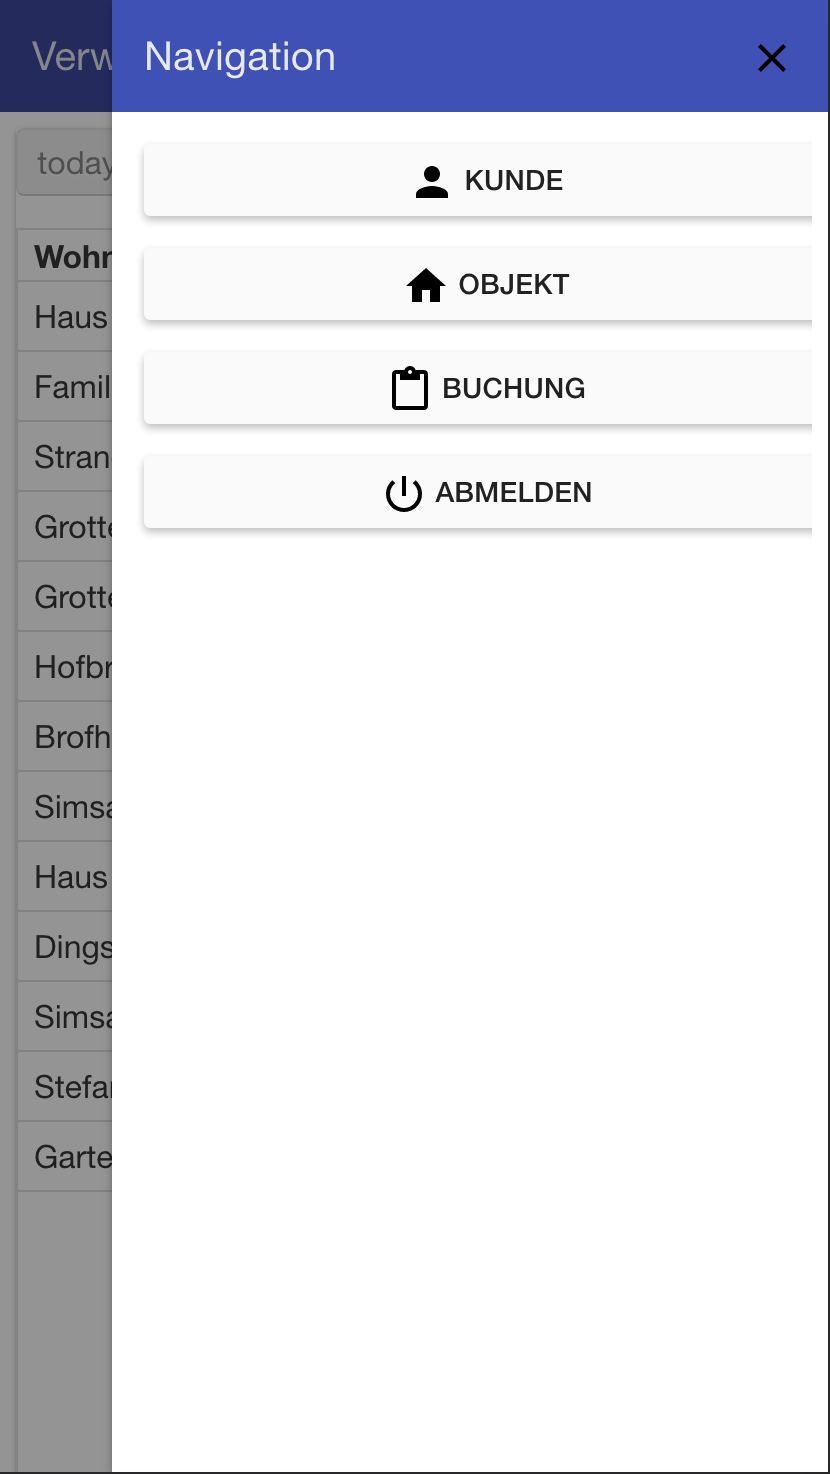
\includegraphics[width=\linewidth]{images/frontend_header_small_navigation.png}
        \label{frontend_header_small_navigation}
        \caption{Seitennavigation auf Mobilgeräten}
    \end{minipage}
\end{figure}


\subsection{Main}
In der Main befindet sich der eigentliche Kalender, in dem in einer Monatsübersicht die Buchungen dargestellt werden. 
Dieser teilt sich in folgende zwei Bereiche:
\begin{description}
\item[Objektübersicht]\hfill \\
Alle Objekte werden auf der linken Seite in form einer Liste dargestellt.
\item[Buchungsübersicht]\hfill \\ 
Alle Tage des aktuellen Monats werden als Spalten dargestellt. Die Buchungen werden als Blöcke angezeigt und verbinden die einzelnen Tage an denen das Objekt gebucht ist.  
\end{description}

\section{Kunde}
Zusammen mit dem Objekt bildet der Kunde eine Buchung. Für die Kundeninformationen wurden alle Felder aus dem Projektzielen implementiert (Abbildung \ref{frontend_customer_new}). Zudem sind alle Felder ausgenommen der Zusatzinformationen und der Firma Pflicht. Diese werden beim Abschicken des Formulars geprüft, ob sie leer sind. Um die Eingabe des Geburtstages zu vereinfachen wurde jeweils für Tag, Monat und Jahr ein Dropdown-Menü bereitgestellt. Da das Mindestalter für Buchungen 18 Jahre ist, ist das höchste auszuwählende Jahr immer 18 Jahre vom aktuellen aus gerechnet. Alle Zeitangaben werden im UNIX TIMESTAMP gespeichert. Sind alle Felder korrekt ausgefüllt, kann das Formular abgeschickt werden. Sobald die \texttt{submit} Funktion im Controller aufgerufen wird, werden alle Felder aus dem View in einem \texttt{customer} JSON-Objekt gespeichert. Diese werden dem \texttt{Customer} Model übergeben und das Dialog geschlossen. 

\begin{lstlisting}[language=JavaScript, label=code_exampleRegistrationRequest, caption=Beispielhafte Antwort auf eine Registrierungsanfrage]
		$scope.submit = function () {
            $scope.birthday = new Date($scope.yearOfBirth + '-' + $scope.monthOfBirth + '-' + $scope.dayOfBirth).getTime();
            var customer = new Customer({
                Company: $scope.company,
                FirstName: $scope.firstname,
                LastName: $scope.lastname,
                BirthDate: $scope.birthday,
                Street: $scope.street,
                City: $scope.city,
                ZipCode: $scope.zipcode,
                Email: $scope.email,
                Phone: $scope.phone,
                Custom: $scope.custom,
                Id: $scope.customerID || undefined
            });
            Customers.upsert(customer);
            $scope.hide();
            $rootScope.$broadcast('showToast');
        };
\end{lstlisting}

Soll ein bestehender Kunde bearbeitet werden (Abbildung \ref{frontend_customer_edit}) muss dieser zunächst über das in Abbildung \ref{frontend_customer_search} gezeigte Suchfeld ermittelt werden. Mit einem Klick auf das Lupensymbol im Kopfbereich des Dialog wird die Suchleiste ein oder ausgeblendet. Sobald das Suchfeld fokussiert wird, wird eine Funktion im Controller angestoßen, welche alle Kunden mit Vor und Nachname als Auswahlmöglichkeit auflistet. Dafür wird die Liste aller Kunden im Model aus der Datenbank angefordert. Dieses Liefert ein Array mit allen Kundenobjekten. Bei einer hohen Anzahl an Kunden kann sich die Suche schwierig gestalten. Aus diesem Grund kann der Kunde durch eintippen von Buchstaben gefiltert werden. Jeder weitere Buchstabe schränkt die Suche nach dem Kunden ein und es werden nur Kunden angezeigt dessen Nachname die eingegebene Zeichenkette beinhalten. 

\begin{figure}[H]
\centering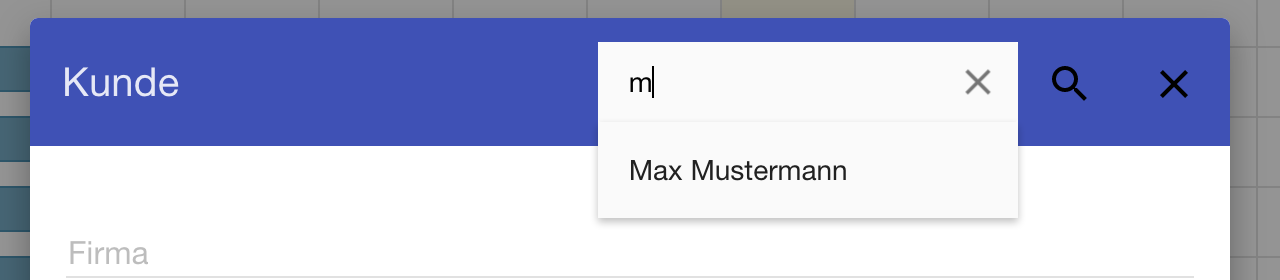
\includegraphics[width=0.5\textwidth]{images/frontend_customer_search.png}
\caption{Kundensuche}
\label{frontend_customer_search}
\end{figure}

\begin{figure}[H]
    \centering
    \begin{minipage}[t]{0.49\linewidth}
        \centering
        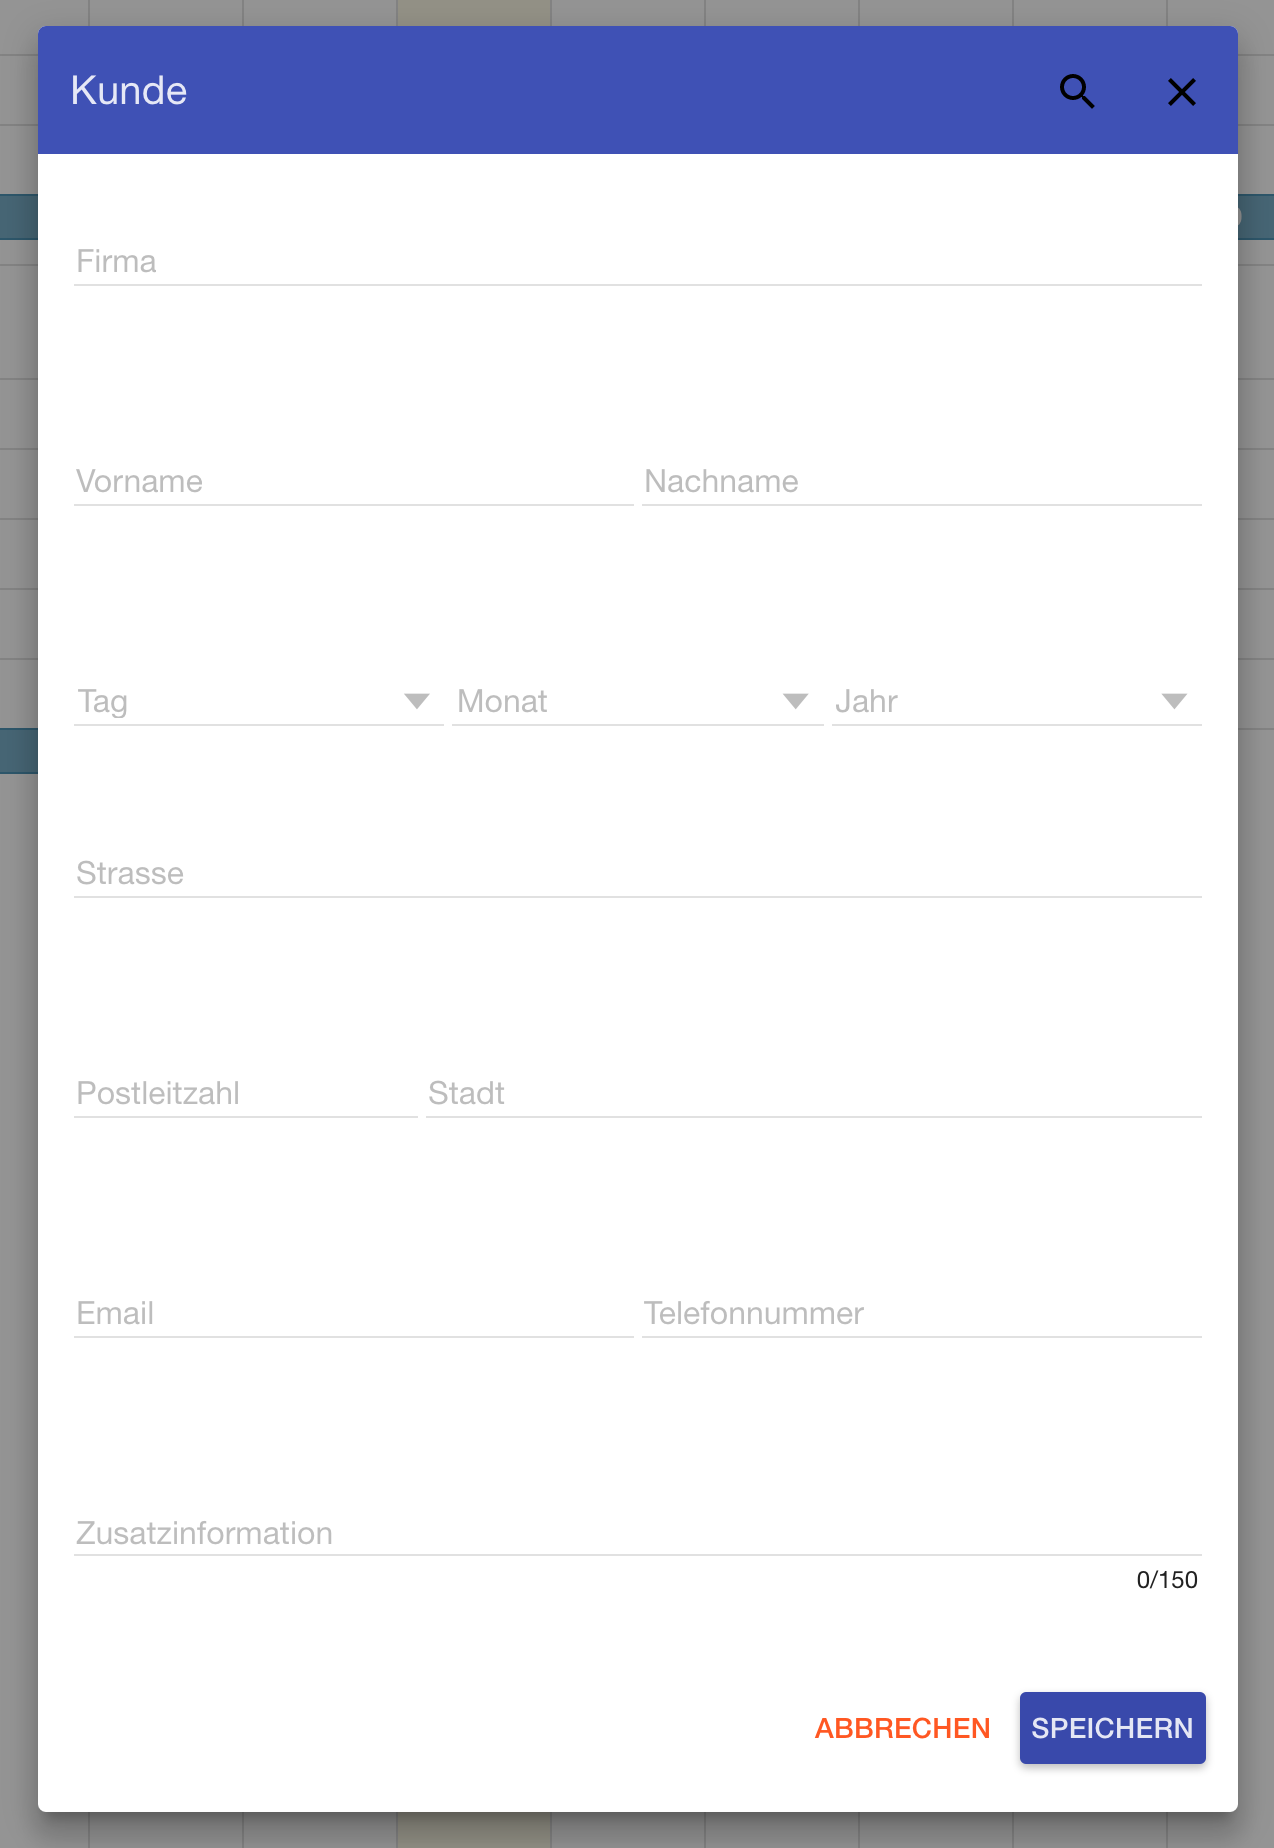
\includegraphics[width=\linewidth]{images/frontend_customer_new.png}
        \label{frontend_customer_new}
        \caption{Neuen Kunden erstellen}
    \end{minipage}% <- sonst wird hier ein Leerzeichen eingefügt
    \hfill
    \begin{minipage}[t]{0.49\linewidth}
        \centering
        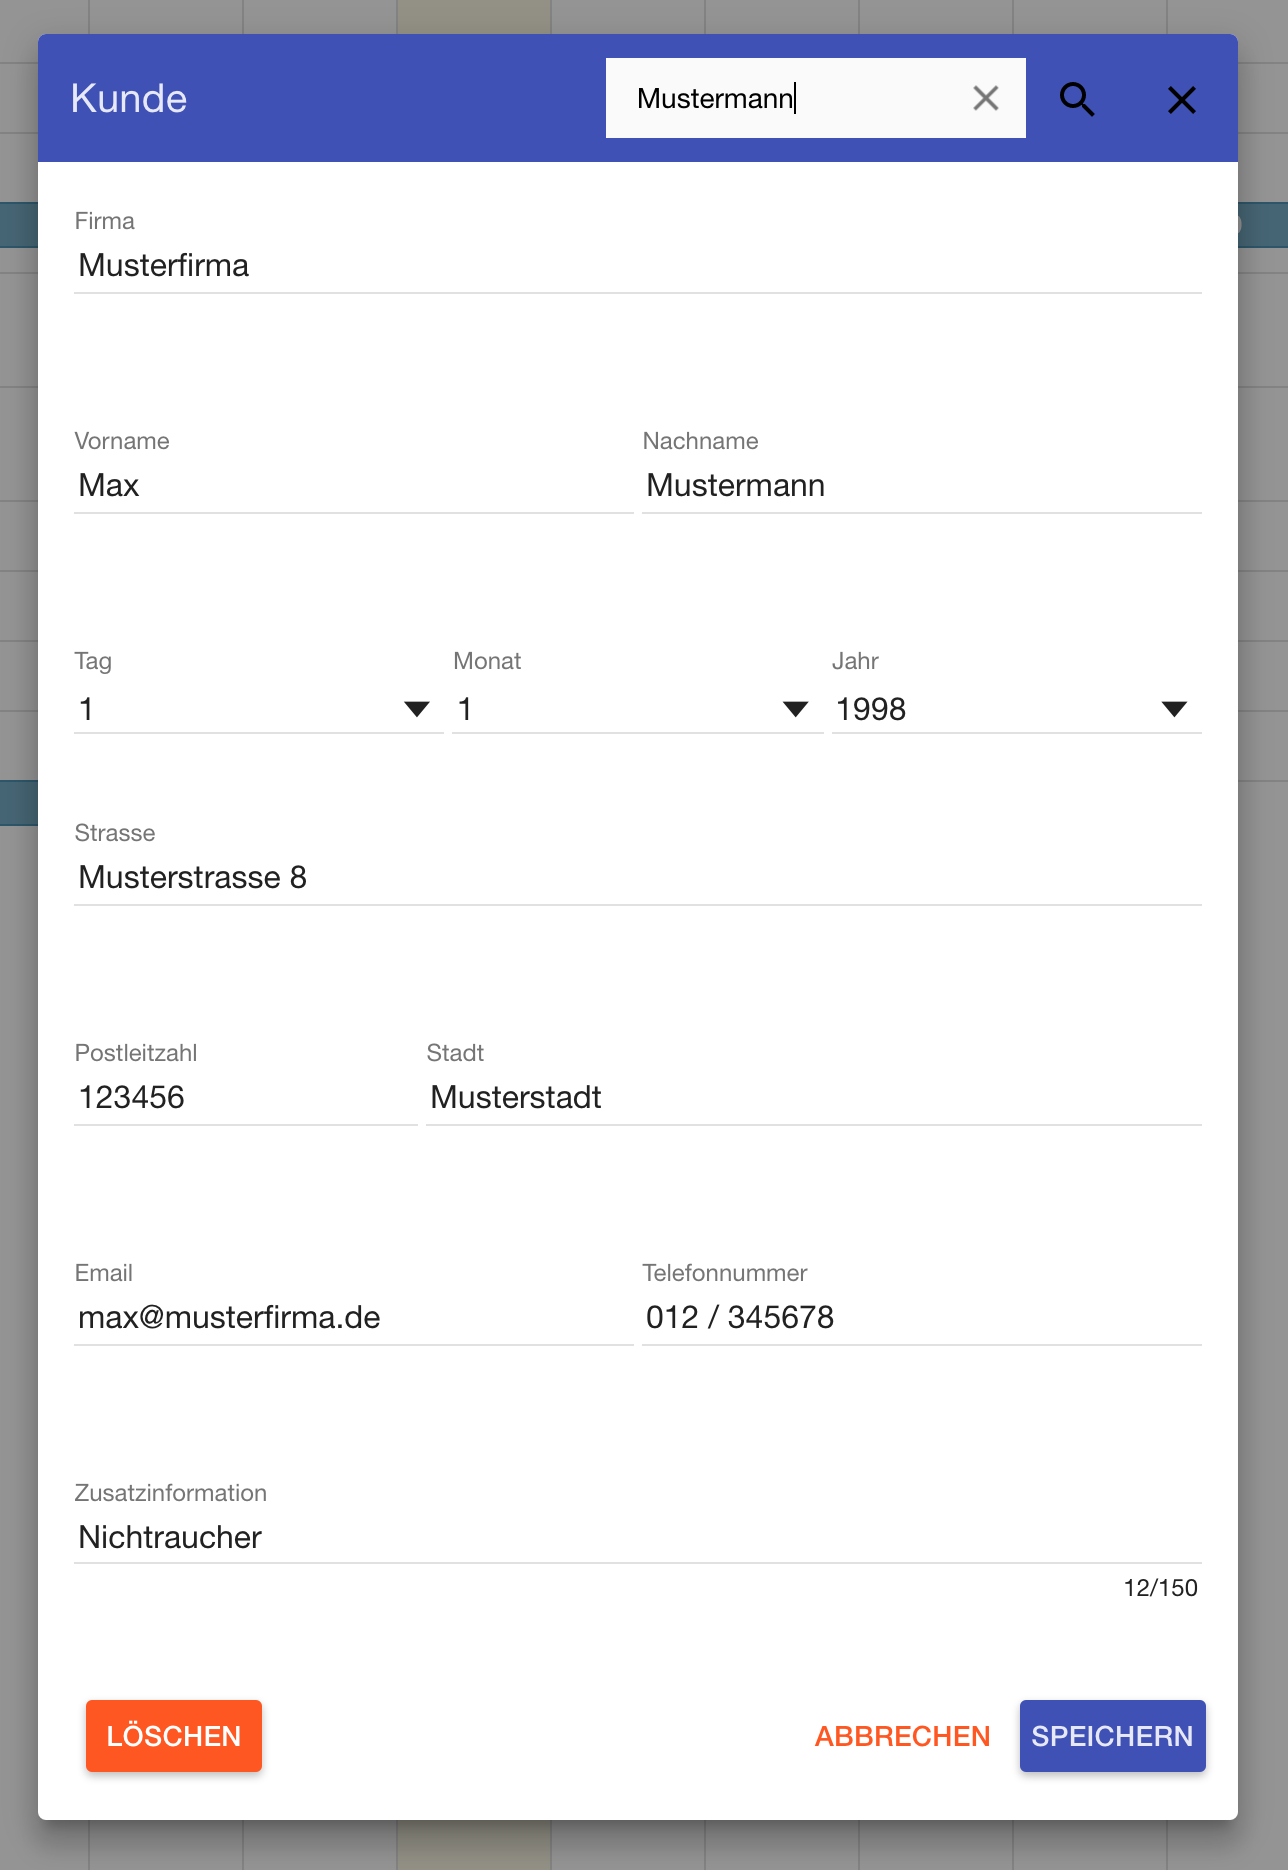
\includegraphics[width=\linewidth]{images/frontend_customer_edit.png}
        \label{frontend_customer_edit}
        \caption{Kunden bearbeiten}
    \end{minipage}
\end{figure}

Wurde ein Kunde ausgewählt, werden alle Daten aus dem JSON-Objekt ausgelesen und in die jeweiligen Input Felder eingefügt. Gleichzeitig wird ein Button zum löschen angezeigt. Um bei der Löschung einem Fehler vorzubeugen muss zusätzlich noch ein Dialog bestätigt werden. Ist das der Fall übergibt der Controller dem Model die UUID des Kunden in einer \texttt{delete} Funktion. 
%TODO delete customer in model

Wenn Daten verändert wurden können diese wie auch beim Hinzufügen eines neuen Kunden ganz normal bestätigt werden. Im Controller wird die \texttt{upsert} Funktion des Model aufgerufen. Je nachdem, ob es sich dabei um einen bestehenden Eintrag in der Datenbank handelt oder der Eintrag bereits vorhanden ist wird ein \texttt{Update} oder \texttt{Insert} durchgeführt. 

Soll weder ein neuer Kunde hinzugefügt noch ein bestehender bearbeitet werden kann das Dialog über den \grqq Abbrechen\glqq  Button, das \grqq X\glqq  oder einen Klick ausserhalb des Dialogs geschlossen werden. Für den Controller ist das ein und die selbe Funktion. Dieser ruft die \texttt{hide} Methode des Dialogs auf und das Dialogfenster wird ausgeblendet. Dabei werden auch alle Daten aus den Feldern entfernt.


\section{Objekt}
Als Objekt wird eine Ferienwohnung oder Haus bezeichnet. Wie auch beim Kunden können bei einem Objekt verschiedene Informationen gespeichert werden. Die beiden Felder aus den Projektzielen wurden implementiert (Abbildung \ref{frontend_resource_new}). Dazu gehört die Eingabe des Namens und die Personenanzahl in ein Textfeld. Wird das Feld fokussiert und ohne Eingabe verlassen erscheint eine Fehlermeldung mit dem Hinweis,dass das Feld auszufüllen ist (Abbildung \ref{frontend_resource_fail}). Wird dieser Hinweis ignoriert und der Nutzer versucht das Formular abzuschicken überprüft der View, ob alle als Pflicht gekennzeichneten Felder ausgefüllt wurden und der \texttt{submit} Button gedrückt wurde. Ist eines dieser Angaben \texttt{false} wird das Formular erst gar nicht abgeschickt.

\begin{figure}[H]
    \centering
    \begin{minipage}[t]{0.49\linewidth}
        \centering
        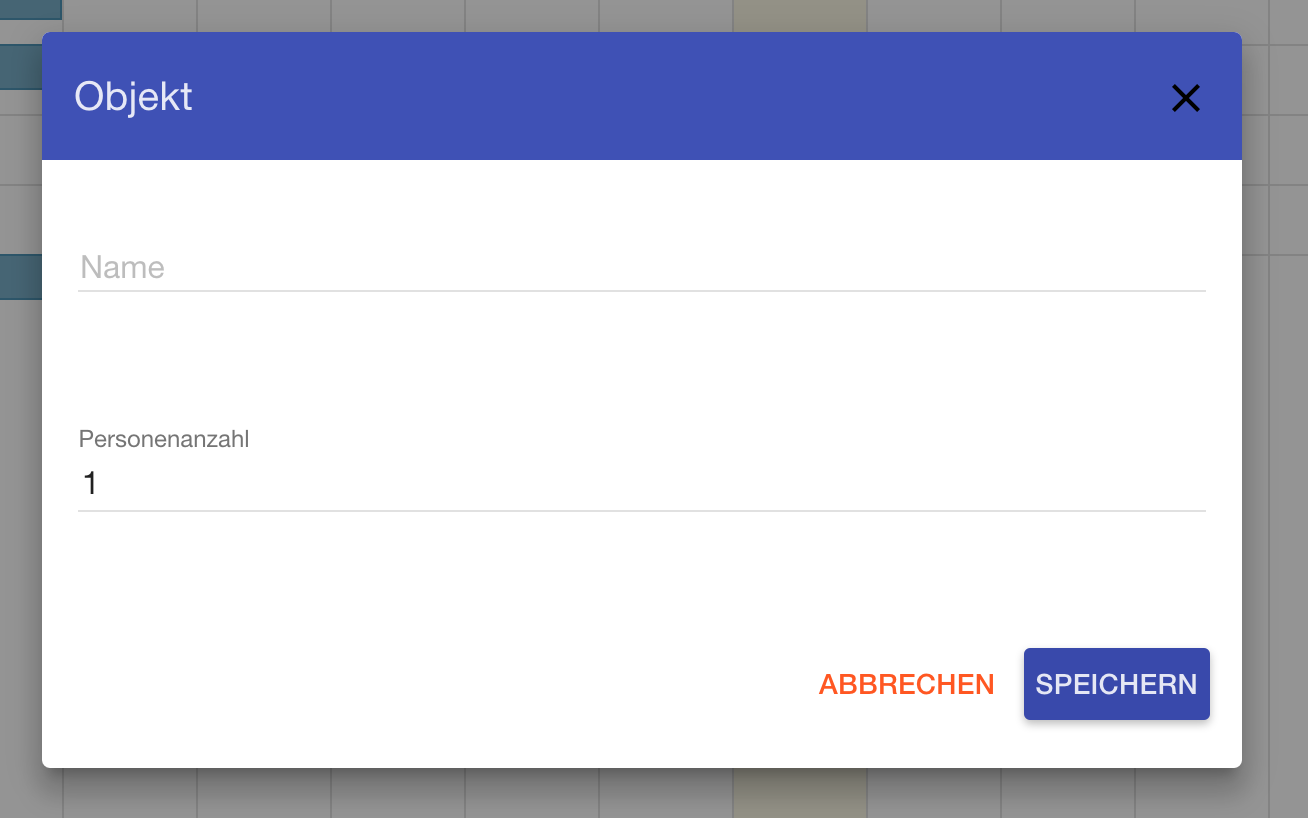
\includegraphics[width=\linewidth]{images/frontend_resource_new.png}
        \label{frontend_resource_new}
        \caption{Objekt erstellen}
    \end{minipage}% <- sonst wird hier ein Leerzeichen eingefügt
    \hfill
    \begin{minipage}[t]{0.49\linewidth}
        \centering
        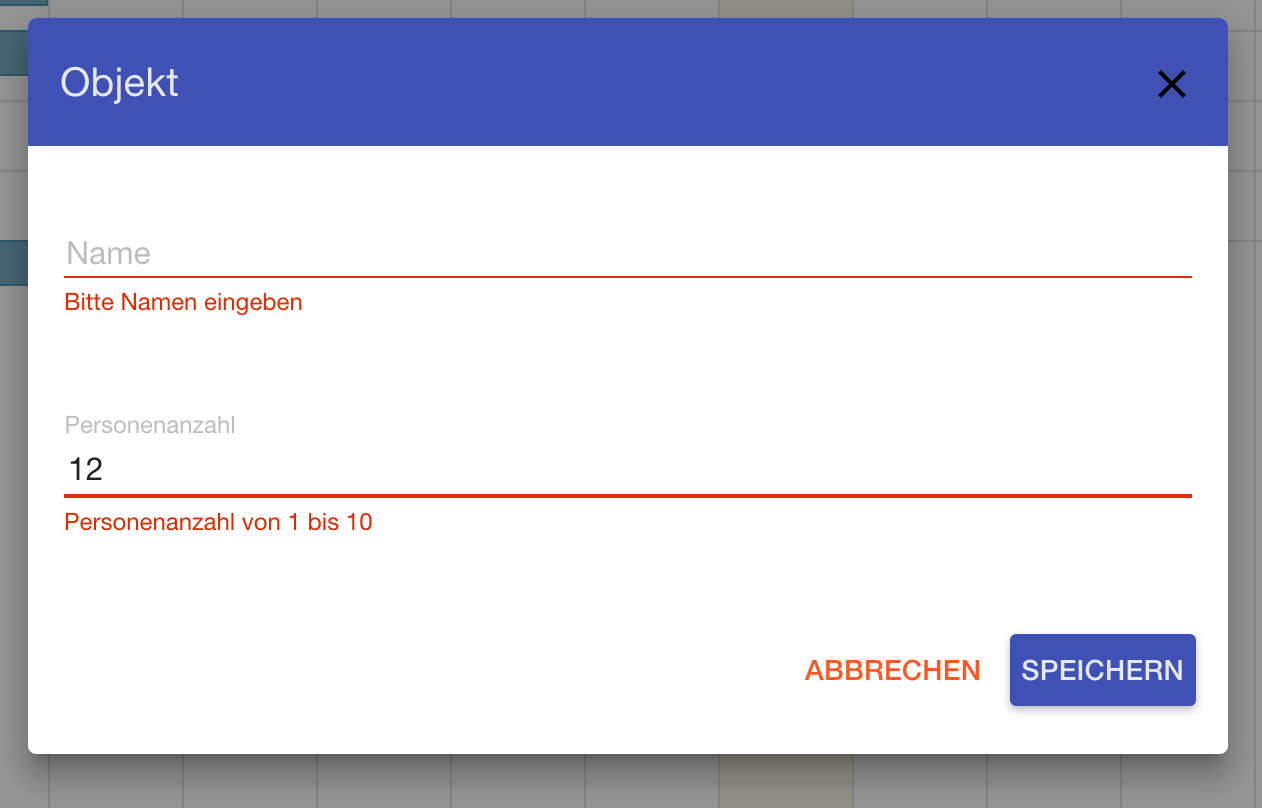
\includegraphics[width=\linewidth]{images/frontend_resource_fail.png}
        \label{frontend_resource_fail}
        \caption{Objekt bearbeiten}
    \end{minipage}
\end{figure}


 Auch bei der Angabe der maximalen Personenanzahl wurde darauf geachtet Falscheingaben abzufangen. Standardmäßig ist eine Mindestpersonenanzahl von 1 eingestellt. Der Nutzer hat die Möglichkeit mit Hilfe von Pfeilen den Wert zu Verändern. Die Maximale Anzahl von Personen ist 10 pro Objekt. Da es auch möglich ist Manuell eine Zahl einzugeben wird ebenfalls überprüft, ob sich die Zahl zwischen 1 und 10 befindet. Ist dies nicht der Fall wird ein Hinweis ausgegeben und das Formular kann nicht abgeschickt werden. Sind alle Angaben korrekt und der \texttt{submit} Button wird betätigt, wird das Formular abgeschickt. Im Controller wird eine Funktion aufgerufen in der die Daten aus den Feldern in ein JSON-Objekt gespeichert werden. Dieses wird der \texttt{upsert} Methode des Models übergeben. Die Überprüfung der Personenanzahl findet im View statt. 
 
 \begin{lstlisting}[language=HTML, label=code_exampleRegistrationRequest, caption=Beispielhafte Antwort auf eine Registrierungsanfrage]
		<input required type="number" step="any" name="rate" ng-model="size" min="1" max="10"  />
            <div ng-messages="resourceForm.size.$error">
                <div ng-message="required">Personenanzahl von 1 bis 10</div>
            </div>
\end{lstlisting}
 
 

Um ein bereits existierendes Objekt bearbeiten zu können muss dies anders als bei den Kunden in der Auflistung im Kalender ausgewählt werden (Abbildung \ref{frontend_resource_edit}). Auch hier werden die Daten anhand der UUID aus der Datenbank geladen und in die Felder eingefügt. Zusätzlich wird der Button zum Löschen des Objektes angezeigt. Die Besonderheit bei der Änderung von Daten ist eine Eigenschaft im JSON-Objekt in dem die Informationen der Felder gespeichert werden. Neben dem Namen und der Personenanzahl wird die ID des Objektes gespeichert. Ist, wie bei einer Änderung, bereits eine UUID vorhanden, wird diese als Wert gespeichert. Wird ein Objekt neu hinzugefügt, ist die ID \texttt{undefined}. Diese Information wird in der \texttt{upsert} Methode des Models abgefragt und dementsprechend ein neues Objekt hinzugefügt oder ein bestehendes aktualisiert.



\begin{figure}[H]
\centering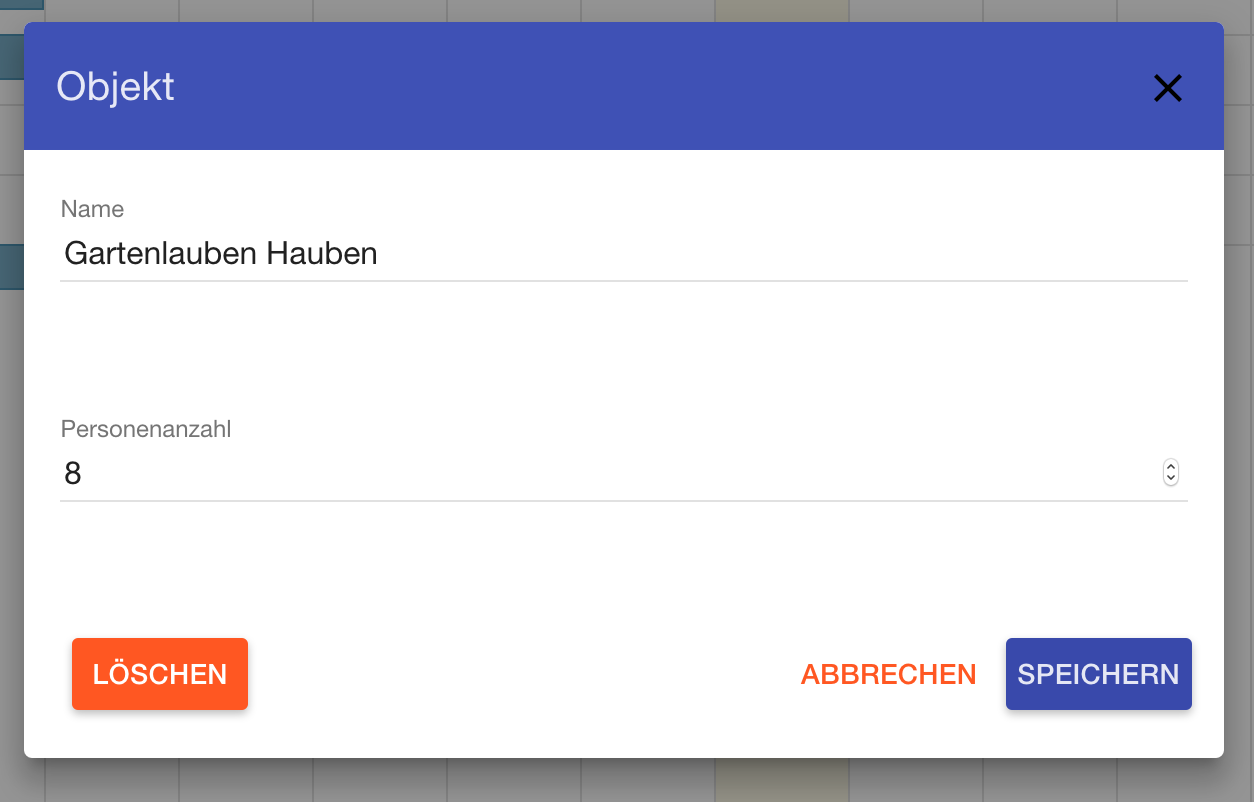
\includegraphics[width=0.5\textwidth]{images/frontend_resource_edit.png}
\caption{Eingabefehler bei Objekt}
\label{frontend_resource_edit}
\end{figure}

%TODO how works upsert at model

  
\section{Buchung}
Eine Buchung ist ein Zusammenschluss aus Kunde, Objekt, Personenanzahl, Startdatum und Enddatum. Wie bei der Bearbeitung von Kunden, kann der Nutzer den Kunden über ein Suchfeld filtern und Auswählen. In diesem Fall gibt es die selbe funktioniert für das Objekt. 

%TODO load data from model

Wenn eine neue Buchung hinzugefügt wird, wird zunächst die Auswahl der Personenanzahl ausgeblendet (Abbildung \ref{frontend_booking_new}). Erst wenn ein Objekt im Suchfeld ausgewählt wurde, wird die Auswahl in form eines Dropdown-Menüs im View angezeigt. Im Controller wird vorher die maximale Personenanzahl des ausgewählten Objektes aus dem JSON-Objekt entnommen und somit die zur Auswahl stehenden Zahlen ermittelt. So zeigt das Dropdown-Menü nur genau die Anzahl von Personen an die dieses Objekt zur Verfügung stellt. Für das Startdatum und Enddatum wurden, anders als beim Kunden, ein Datepicker bereit gestellt, der es dem Nutzer erlaubt das Datum durch einfache Auswahl in einem Kalender festzulegen (Abbildung \ref{frontend_booking_calender}). Für diesen ist Standardmäßig das aktuelle Datum eingestellt.

\begin{figure}[H]
    \centering
    \begin{minipage}[t]{0.49\linewidth}
        \centering
        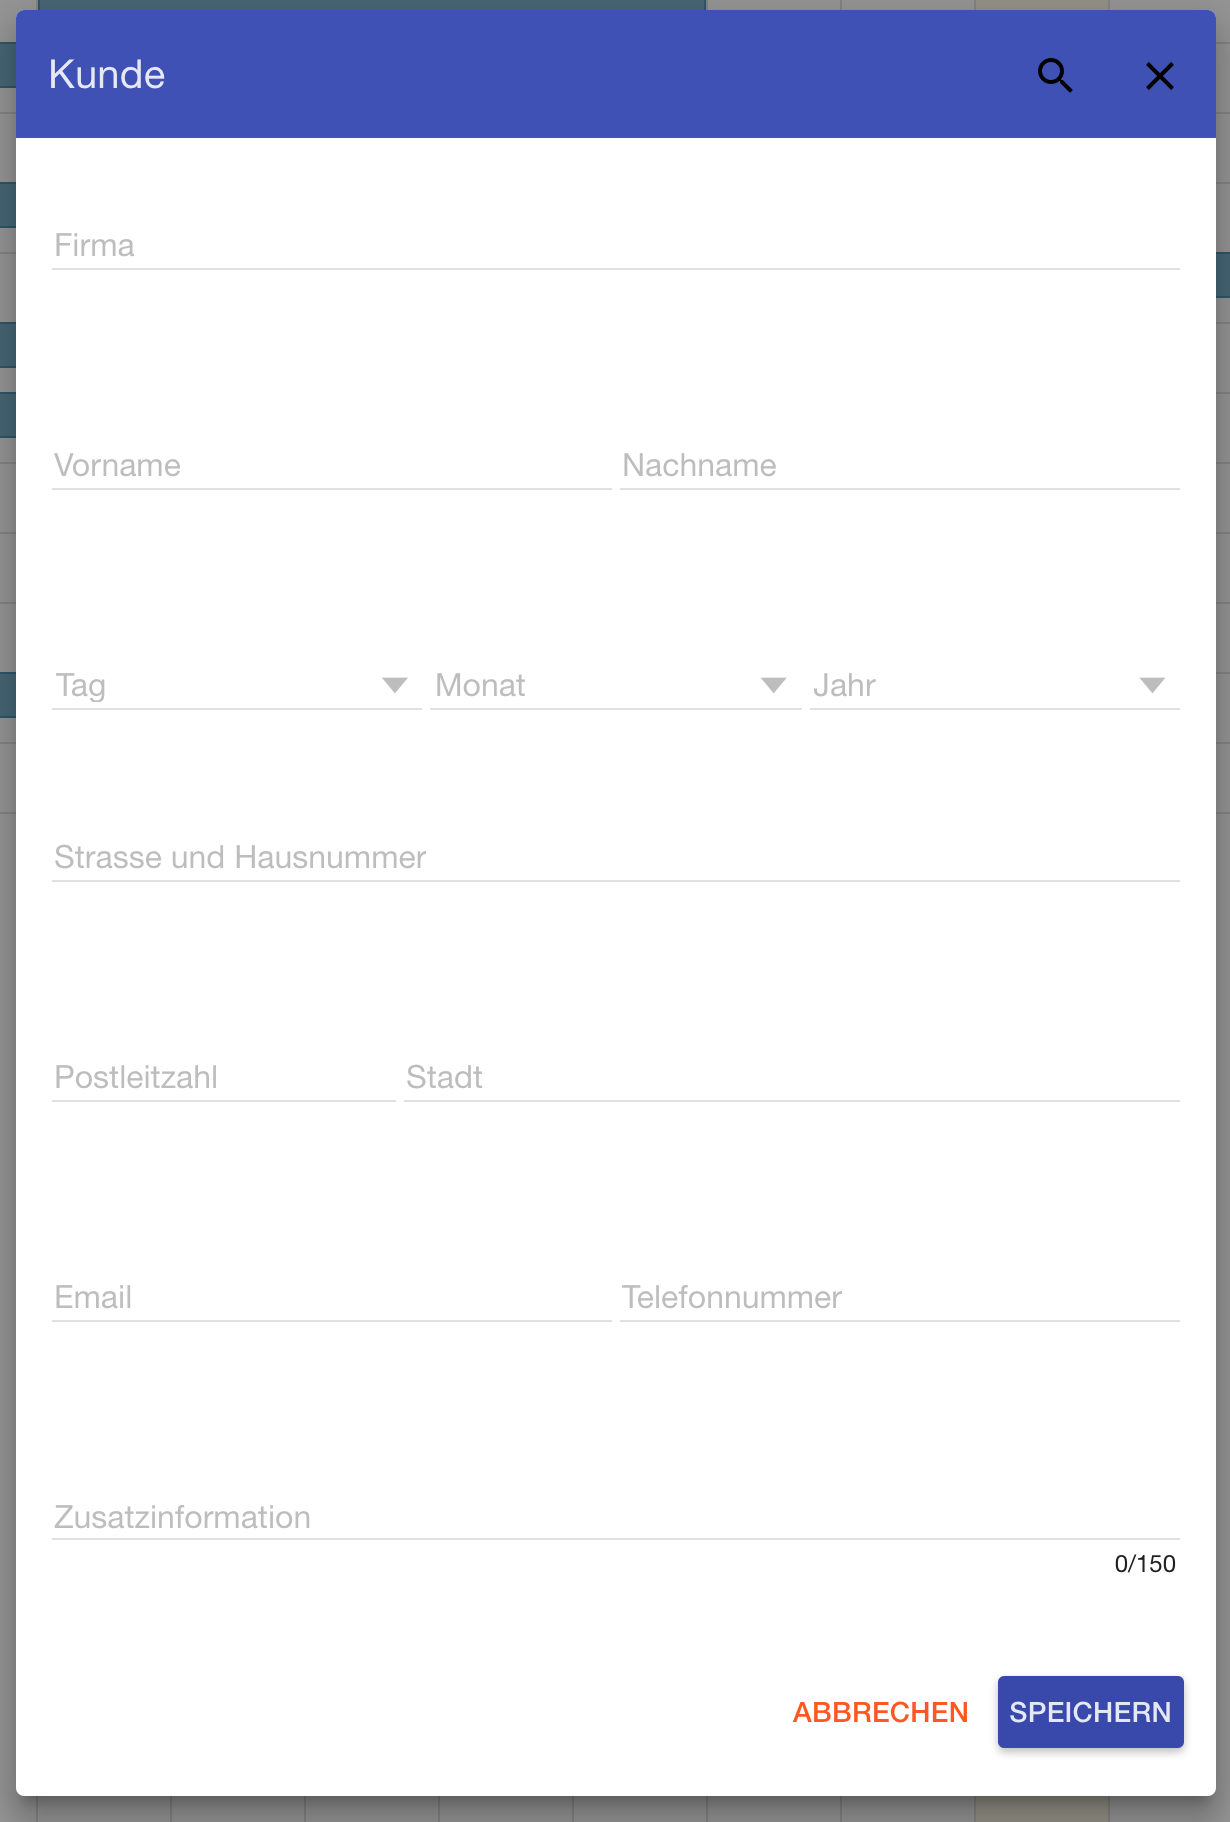
\includegraphics[width=\linewidth]{images/frontend_booking_new.png}
        \label{frontend_booking_new}
        \caption{Objekt erstellen}
    \end{minipage}% <- sonst wird hier ein Leerzeichen eingefügt
    \hfill
    \begin{minipage}[t]{0.49\linewidth}
        \centering
        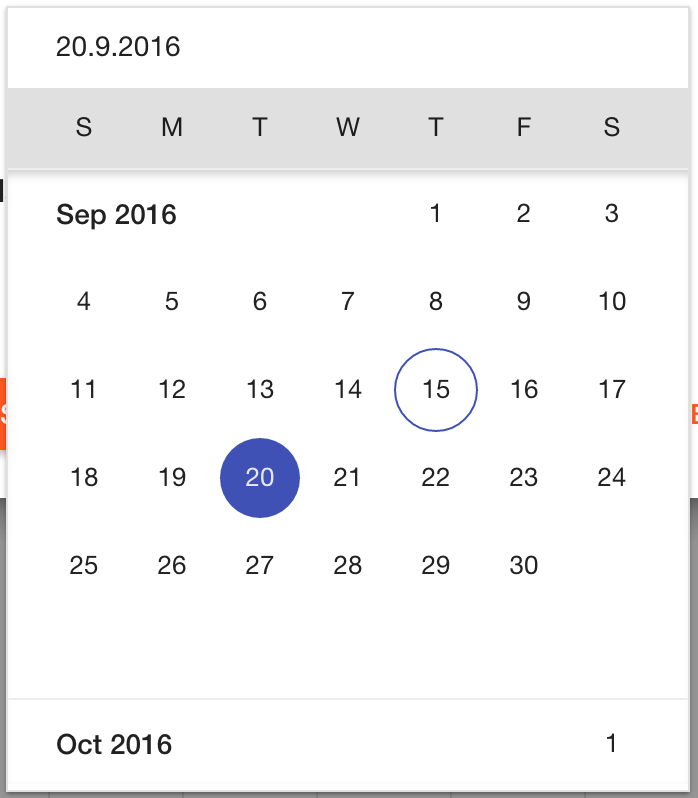
\includegraphics[width=\linewidth]{images/frontend_booking_calender.png}
        \label{frontend_booking_calender}
        \caption{Auswahl des Datum}
    \end{minipage}
\end{figure}

Um eine Buchung bearbeiten zu können muss diese, anders als beim Kunden oder Objekt, zunächst in der Buchungsübersicht gesucht werden. Hier wird die Personenauswahl angezeigt und ist mit dem eingetragenem Wert vordefiniert. Auch hier besteht die Möglichkeit, durch den angezeigten Löschen-Button die Buchung aus der Datenbank zu entfernen (Abbildung \ref{frontend_booking_delete_dialog}).  

\begin{figure}[H]
    \centering
    \begin{minipage}[t]{0.49\linewidth}
        \centering
        
\includegraphics[width=\linewidth]{images/frontend_booking_delete_dialog.png}
        \label{frontend_booking_delete_dialog}
        \caption{Objekt erstellen}
    \end{minipage}% <- sonst wird hier ein Leerzeichen eingefügt
    \hfill
    \begin{minipage}[t]{0.49\linewidth}
        \centering
        
\includegraphics[width=\linewidth]{images/frontend_toast.png}
        \label{frontend_toast}
        \caption{Objekt Fehlereingabe}
    \end{minipage}
\end{figure}


Wird ein Dialog bestätigt, wird erscheint für drei Sekunden am oberen rechten Fensterrand ein Nachricht (Abbildung\ref{frontend_toast} sky). Ein sogenannter Toast fährt herunter und zeigt die Erfolgsmeldung und einen Button zum schließen an. In der mobilen Ansicht fährt der Dialog, in voller Bildschirmbreite, von unten herein. 

\section{Kalender}

%TODO write text about the main calender

\section{Backend}
% Documents\Medieninformatik\Master\EvA\eva-ss2016
Für die entwickelte Anwendung kommt die Plattform \"Firebase\" von Google zum Einsatz.
\\
Diese stellt neben einer Echtzeit-Datenbank, Authentifizierungs-Funktionen und Cloud-Messaging, auch Speicherplatz sowei ein Hosting für Web-Apps zur Verfügung.
In der Basis-Version, welche auch für die Entwicklung der vorliegenden Anwendung verwendet wurde, ist die Nutzung kostenlos. Für höhere Leistungsansprüche stehen kostenpflichtige Pakete zur Verfügung.\\
Im nachfolgenden erfolgt eine Erläuterung der einzelnen Komponenten, die von der Anwendung benutzt werden.

\subsection{Echtzeit-Datenbank}
Bei der von Firebase verwendeten Datenbank handelt es sich um eine sog. NoSQL-Datenbank. Im Gegensatz zu anderen Datenbank-Systemen wie bspw. MySQL, erfolgt die Abspeicherung der Daten dokumentenbasiert im JSON-Format.
Dokumentenbasiert bedeutet, dass einzelne Einträge der Datenbank als Objekte abgelegt werden. Dabei sind diese Objekte von Grund auf nicht an Schemata gebunden und können beliebige Strukturen beinhalten.
Dabei können auch Objekte, die von ihrer Gruppierung her gleich sind, unterschiedlich viele und anders typisierte Daten beinhalten.\\


\subsubsection{Organisation}
Die Bennenung der Gruppen von Datensätzen ist von Firebase sehr flexibel gestaltet und ermöglicht beliebige Namen.
Wie bereits in dem Kapitel Models erläutert, existieren die folgenden Gruppen:
\begin{itemize}
\item bookings
\item customers
\item resources
\end{itemize}

Jede Gruppe kann beliebig viele Untergruppen oder Objekte besitzen. Dabei gibt es keine Einschränkungen.\\
Die Daten in den Objekten sind in der JSON-typischen Key:Value-Notation abgelegt.
Identifiziert werden die Objekte über einzigartige Schlüssel, die als ID fungieren.
Über diese Schlüssel lassen sich später in der Anwendung einzelne Objekte direkt abfragen.
Weiterhin können über diese Keys Beziehungen zu anderen Objekten aufgebaut werden.
Behandelt werden diese Schlüssel wie Zeichenketten und erfahren somit keiner speziellen Behandlung sofern sie als Werte eines Objektes abgelegt sind.

\subsubsection{Zugriffsverwaltung}
Firebase bietet dem Administrator sehr flexible Zugriffsregeln, mit welchen die exakte Steuerung von Lese- und Schreibzugriffen möglich ist.
Die Ausgangskonfiguration beschränkt das Lesen und Schreiben von Datensätzen auf eingeloggte Benutzer. Auf die Authentifizierung-Möglichkeiten wird in dem Kapitel Authentifizierung eingegangen.\\
Wie die Organisation der Daten in der Datenbank im JSON-Format angelegt ist, werden auch die Regeln als JSON-Notation hinterlegt.
\textt{\{
         "rules": \{
           ".read": "auth != null",
           ".write": "auth != null"
         \}
       \}}
Der hier dargestellte Konfigurationsabschnitt zeigt die Regeln für den Lese- und Schreibzugriff auf die gesamte Datenbank. Demnach dürfen nur eingeloggte Benutzer lesen und schreiben. Firebase ermöglicht es, für jede Gruppe eine separate Konfiguration zu generieren.
Entscheidend dafür, ob Daten gelesen oder geschrieben werden dürfen ist das Ergebnis des Ausdrucks bei \textt{.read} und \textt{.write}. Diese müssen jeweils bei ihrer Ausführung zu einem boolschen Wert evaluieren. Dabei können diese Regeln eine beliebige
Komplexität aufweisen.
In der vorliegenden Anwendung wurde auf eine komplexe und spezifische Konfiguration verzichtet, da der Anwendungsfall keine spezielle Behandlung von verschiedenen Benutzern fordert.
Alle Datensätze können nur von authentifizierten Benutzern gelesen und geschrieben werden.

\subsubsection{Lesen, Schreiben, Echtzeit-Synchronisation}
Der entscheidende Punkt bei der Auswahl der Backend-Platform war der Aspekt der Echtzeit-Synchronisation der Datenbank zwischen den angemeldeten Clients.
Um eine Echtzeit-Anwendung zu realisieren, sollten Daten, die bei Client A generiert, verändert oder gelöscht wurden, bei Client B ohne ein Neuladen der gesamten Anwendung aktualisiert werden.\\
Diese Synchronisation wird von Firebase durch die Verwendung der Web-Socket-Technologie ermöglicht. Technisch gesehen basiert dies auf dem Austausch von Nachrichten. Dabei baut die Anwendung eine konstante Verbindung
zu dem Firebase-Server auf. Sobald eine Daten-Transaktion abgeschlossen ist, sendet Firebase eine Nachricht an alle verbundenen Clients. Bei der Entwicklung kann der Entwickler entscheiden, ob er auf etwaige Nachrichten reagieren möchte.
Bei den Nachrichten wird zwischen fünf verschiedenen Ereignissen unterschieden\:
\begin[itemize]
\item{\textbf{value} Allgemeine Änderung an einer Gruppe}
\item{\textbf{child_added} Einer Grupper wird ein neues Element hinzugefügt}
\item{\textbf{child_changed} In einer Grupper ändert sich ein eizelnes Kind-Element}
\item{\textbf{child_removed} Ein Element wird aus einer Gruppe entfernt}
\item{\textbf{child_moved} Die Reihenfolge eines Kind-Elements verändert sich}
\end{itemize}

Wie dieses Feature in die entwickelte Anwendung integriert wurde, wird im Kapitel Collections genauert erläutert.

\subsection{Authentifizierung}
Bei fast jeder zu entwickelnden Anwendung steht das Thema Nutzer-Authentifizierung auf dem Plan. Standardmäßig erfolgen Implementierungen, die Benutzer mit Hilfe von Email/Benutzernamen und Passwort authentifizieren.
Leider kann es hierbei immer wieder zu Fehlern in der Entwicklung oder im Design kommen, sodass es u.U. möglich ist, Zugang zu gesperrten Bereichen oder Daten zu erlangen.
Um dem Entwickler einerseits dieses Risiko zu nehmen und andererseits erheblichen Implementierungs-Aufwand zu ersparen, bietet Firebase auch einen Auhentifizierungs-Service an.
Per Standard ist das Email-Passwort-Verfahren aktiviert. Zudem bietet Firebase auch die Authentifizierung mithilfe von Accounts von Facebook, Google, Twitter und GitHub an. Dabei werden OAuth 2.0 und OpenID Connect verwendet. Weiterhin lassen sich
beliebig viele weitere OAuth-Services hinzufügen.\\

In der vorliegenden Anwendung wurde das Email-Passwort-Verfahren verwendet, da analog zum Zugriffsschutz auch hier nur ausgewählte Benutzer Zugriff auf die Anwendung erhalten und somit
keine Authentifizierung über weitere Dienste nötig sind.
\\
Wie diese Anmeldung in der Anwendung abläuft, wird im entsprechenden Kapitel im Bereich Frontend erläutert.

\subsection{Weitere Firebase-Funktionen}
Neben den erläuterten Funktionen stellt Firebase zusätzlich Hosting und Datenspeicher, sowie Cloud Messaging, Analytics und Monetarisierungs-Optionen zur Verfügung.
Zudem bietet Firebase sehr gute Vorraussetzungen für schnell wachsende Anwendungen, da über die Web-Konsole schnell und einfach Kapazitäten angefordert werden können.
\subsection{Technische Umsetzung der Datenbank-Anbindung}
Um die Arbeit mit Datensätzen und Daten-Listen zu erleichtern, wurde ein System nach einem Model-Collection-Pattern entwickelt.
Demnach sind einzelne Datensätze über Models organisiert. Diese Models werden in typisierten Collections zusammengefasst.
Im nachfolgenden werden der Aufbau und die Funktionsweise beider Konstrukte erläutert.

\subsubsection{Models}

Als Model bezeichnet man eine Klasse, die die Struktur eines Objektes beschreibt. Ein Model hat einen Constructur, über welchen sich ein neues Objekt dieses Types generieren lässt.
Im Fall der vorliegenden Anwendung bilden drei verschiedene Models die Datenstruktur des Systems ab.\\
Dazu gehören:
\begin{description}
\item[Booking]\hfill \\
Hält eine Buchung
\item[Customer]\hfill \\
Beschreibt den Kunden
\item[Resource]\hfill \\
Beschreibt das vermietete Objekt
\end{description}

Über ein Model lässt sich ein Objekt eines spezifischen Types generieren.
Innerhalb der AngularJS-Anwendung wird das Model als Factory-Service implementiert. Dies ermöglicht es, beliebig viele Instanzen dieses Models zu generieren.
Im nachfolgenden der Aufbau des Resource-Models:

\begin{lstlisting}[language=Javascript, label=code_ResourceModel, caption=Hauptteil des Reosurce-Models]
angular.module('bookingCalendarApp')
    .factory('Resource', function ($log) {
        function Resource(properties){

            var self = this;

            this.Id    = undefined;
            this.Size  = undefined;
            this.Name  = undefined;

            function extend(properties){
                [...]
            }

            extend(properties);

        }

        return Resource;
    });
\end{lstlisting}

Wesentlicher Bestandteil des Models sind seine Properties, welche die beschreibbaren Felder darstellen. Bei jeder Instanziierung wird die Methode \texttt{extend\(\)} aufgerufen, welche die
übergebenen Werte auf das Model überträgt.
Innerhalb der Anwendung können Models in allen möglichen Komponenten verwendet werden. Zu beachten ist, dass es anders als bei komplett objektorientierten Sprachen wie bspw. Java,
keine Getter- oder Setter-Methoden gibt und die Properties des Models alle als Public angesehen werden können.


\subsubsection{Remote Objects}
Der Service \texttt{RemoteObjects} agiert als Factory zum Erstellen einer Collection für spezifische Models. Sie ist über einen Angular-Service als Singleton-Klasse implementiert und besitzt
 nur eine Mthode zum Generieren einer neuen Collection.

 \begin{lstlisting}[language=Javascript, label=code_RemoteObject, caption=Code des RemoteObjects-Service]
 angular.module('bookingCalendarApp')
     .service('RemoteObject', function (Collection) {
         var service = {};
         service.createCollection = function(name, path, Model, realtime){

             if(!name || !path || !Model){
                 throw new Error('remoteObject:: Missing parameter in Object')
             }
              return new Collection({
                 name : name,
                 path : path,
                 realtime : realtime,
                 Model : Model
             });
         };
         return service;
     });
\end{lstlisting}

Wie zu sehen, fordert die Factory bei der Instanziierung bis zu vier Parameter. Über den Parameter \texttt{name} wird der Name der Collection bestimmt, \texttt{path} ist der Pfad, unter welchem die Objekte dieses Types
innerhalb von Firebase gefunden werden können, \textt{Model} ist das Model-Objekt und \texttt{realtime} ein Indikator, ob die Collection auf Echtzeit-Updates der Datenbank hören soll.

Rückgabewert der Methode \texttt{createCollection()} ist immer die Collection des jeweiligen Model-Types.
Wie diese Collections funktionieren, wird im nächsten Kapitel erläutert.

\subsection{Collections}

Eine Collection bezeichnet eine Art Sammlung für einen bestimmten Datentypen. Sie stellt Funktionen zur Verfügung, mit welchen der Entwickler einfach Datenbank-Abfragen generieren und Daten speichern kann.
Ebenso wie der RemoteObjects-Service, ist auch eine Collection als Service imlementiert, sodass nur jeweils eine für jedes Model existieren kann.

\subsubsection{Instanziierung}

\subsubsection{Methoden}

\subsubsection[Echtzeit-Anbindung]
\chapter{Fazit}
Die Entwicklung dieses Projektes hat einige sehr interessante Aspekte der interaktiven und innovativen Web-Entwicklung hervorgebracht.
Angefangen bei der Verwendung der Firebase-Platform von Google. Diese bot einen Funktionsumfang, der, im Falle einer Selbstentwicklung,
einem Entwickler einen sehr hohen Aufwand erspart. Zu Beginn ist Firebase kostenlos und ermöglicht auch Studenten, die Platform ohne Kosten zu nutzen.\\
In jedem Fall konnte sich die Plattform für die weitere Nutzung in Uni-Projekten und darüber hinaus empfehlen.
\\
Der entstandene Prototyp funktioniert sehr gut. Vor allem die Synchronisation der Daten zwischen verschiedenen Clients läuft erstaunlich schnell.
Eine Weiterentwicklung des Prototyps ist voraussichtlich nicht vorgesehen
\\
Zusammengefasst lässt sich sagen, dass das Projekt uns persönlich in unseren Interessensgebieten durchaus weitergebracht hat und neue Technologien dadurch zu unserem
Repertoire gehören.\\
Kommende Projekte würden wir wieder mit dieser Technologie-Kombination entwickeln.

%-------------------------------------------------------
% Weitere Verzeichnisse
%-------------------------------------------------------
\pagebreak
{\listoffigures
\raggedbottom
%\pagebreak}
%{\listoftables
%\raggedbottom
\pagebreak}
{\lstlistoflistings
\raggedbottom
\pagebreak}
\printbibliography
\glsaddall
\printglossary[nonumberlist]
\end{document}